\documentclass[11pt,a4paper]{article}
\usepackage{fontspec}
\setmainfont{Source Serif 4}[Path=/home/claude/ref/fonts/, UprightFont=SourceSerif4-Regular.ttf, BoldFont=SourceSerif4-Semibold.ttf, ItalicFont=SourceSerif4-It.ttf]
\setmonofont{IBM Plex Mono}[Path=/home/claude/ref/fonts/, UprightFont=IBMPlexMono-Regular.ttf, BoldFont=IBMPlexMono-Medium.ttf, Scale=0.88]
\usepackage[a4paper,margin=2.4cm]{geometry}
\usepackage{amsmath}
\usepackage{graphicx,booktabs,float,caption,array,xcolor,longtable}
\usepackage{xurl}
\usepackage[hidelinks]{hyperref}
\usepackage[round]{natbib}
\usepackage{setspace}
\setstretch{1.08}
\renewcommand{\topfraction}{0.9}
\renewcommand{\bottomfraction}{0.8}
\renewcommand{\textfraction}{0.1}
\renewcommand{\floatpagefraction}{0.75}
\setlength{\parindent}{0pt}
\setlength{\parskip}{0.55em}
\captionsetup{font=small,labelfont=bf}
\setlength{\bibsep}{3pt}
\urlstyle{same}
\hypersetup{pdftitle={How Old Is Your Neighbourhood?},pdfauthor={Dr Tristan Hotham}}

\begin{document}
\begin{center}
{\Large\bfseries How Old Is Your Neighbourhood? The Age of the Housing Stock in Every Small Area of England and Wales, and the Tree Rings of Its Cities\par}
\vspace{1.2em}
{\large Dr Tristan Hotham\par}
\vspace{0.3em}
{\small Independent researcher\\
ORCID: 0000-0003-4931-9349\\
DOI: https://doi.org/10.5281/zenodo.24113860\par}
\vspace{0.8em}
2026
\end{center}

\begin{quote}
\small
\begin{center}\textbf{Abstract}\end{center}
How old are the homes of England and Wales, area by area, and do cities hold their housing in rings of age, as vintage models of urban growth suggest? I use the Valuation Office Agency's count of every property on the Council Tax lists at 31 March 2025 by build period, published for all 35,672 lower layer super output areas, to map the age of the stock at the finest public scale and to test four hypotheses, written in a plan before any distance was computed, about housing age in the 34 cities of England and Wales with at least 100,000 people. Of homes of known age, 20.8\% predate 1919 and 11.8\% date from 2009 onwards. Within 20 km of the centres, the homes of each successive period from before 1900 to 1965 to 1972 stand on average 4.3\% farther out (95\% CI 3.1 to 5.5), a pattern no placebo centre reproduces. The sequence then reverses: homes built since 2009 stand 9.0\% closer to the centre than homes of 1983 to 1999 (95\% CI 4.9 to 13.0; closer in 26 of 34 cities), and within 1 km of the centres 32\% of homes date from 2009 or later. A linear rise of mean build year with distance fails the pre-specified placebo test. The results hold across nine robustness checks. The stock records survival as well as building, and the data cannot separate the two.

\textbf{Keywords:} housing stock; dwelling age; urban growth; vintage models; recentralisation; Council Tax; England and Wales
\end{quote}

\section{Introduction}
\label{sec:intro}
A city's housing is built slowly and lasts a long time. Each generation adds its homes where land is available at the time, mostly at the edge, and the stock that results carries the history of the city's growth in its layout: an older core, newer rings, and at the fringe the homes of the latest boom. This intuition underlies the vintage models of urban economics, in which a growing city adds rings of housing of successively later dates \citep{harrison1974,brueckner1980,wheaton1982,braid2001}, and the more recent argument that the age of the stock helps explain where rich and poor neighbourhoods form and how they change \citep{rosenthal2008,brueckner2009,rosenthal2015}. Durable housing also shapes how cities decline: homes outlast the demand that called them into being \citep{glaeser2005}.

Despite the importance of building age in these accounts, there has been no simple, complete public map of the age of the housing stock of England and Wales at a fine scale. The Valuation Office Agency (VOA) holds a build period for nearly every property on the Council Tax valuation lists, and since the move to 2021 small-area geographies it publishes the counts for every lower layer super output area (LSOA), an area of about 760 homes on average \citep{voa2025,voa2025bg}. This paper uses those counts to do two things.

First, it describes the age of the housing stock at the finest public scale: the shares of homes built in each of twelve periods from before 1900 to 2009 onwards, in every one of the 35,672 LSOAs, the oldest and newest local authorities, the areas where most homes are new, and how age relates to Council Tax band and property type. The maps and the data are released with the paper.

Second, it tests whether the cities of England and Wales hold their housing in rings of age. I take the 34 places in England and Wales that Natural Earth lists with at least 100,000 people, assign each LSOA within 20 km to its nearest centre, and ask four questions, all specified in a written plan before any distance was computed (Section~\ref{sec:design}). Does the mean build year rise with distance from the centre (H1)? Do the homes of each successive period stand farther out (H2)? Have the newest homes reversed that order, standing closer to the centre than the homes of the 1980s and 1990s (H3)? And do the interwar homes form a ring between the pre-1919 core and the post-war periphery (H4)?

The answers are mixed in an informative way. The ring structure of the twentieth century is strong and consistent: from before 1900 to 1965 to 1972, each successive period's homes stand on average 4.3\% farther from the centre, the order holds in 33 of 34 cities, and centres moved at random by 10 km never produce a pattern as strong. The interwar ring lies where the models put it in 32 of 34 cities. But the newest housing has reversed the direction of growth. Homes built since 2009 stand 9.0\% closer to the centre than the homes of 1983 to 1999, and in the first kilometre around the centres they are the largest single group: 32\% of homes there were built in 2009 or later, and 79\% of homes in those central areas are flats. The simplest test, a linear rise in mean build year with distance, gives a positive slope but fails the placebo test set in advance, because the centre is now among the youngest places in the city and the oldest homes sit in a ring one to two kilometres out. Housing age in English and Welsh cities is thus ordered in rings, but not in a single monotone gradient.

The contribution is threefold: a complete, reproducible small-area description of the age of the housing stock of England and Wales from an administrative source; a pre-specified test of the ring structure predicted by vintage models of urban growth, with a placebo design that separates centre-specific structure from generic spatial patterns; and evidence of recentralisation of new housing at the scale of whole cities. Section~\ref{sec:lit} reviews the background, Section~\ref{sec:data} the data, Section~\ref{sec:design} the design, Section~\ref{sec:results} the results, Section~\ref{sec:robust} the robustness checks and Section~\ref{sec:discussion} the discussion and limitations.

\section{Background}
\label{sec:lit}
\subsection{Vintage, durability and the ages of urban housing}
In the standard account of urban structure, housing costs fall with distance from the centre, and falling commuting costs let cities spread outwards into suburbs \citep{ioannides2008}. Static versions of this account say nothing about building age, and real cities also grow discontiguously, leaving land to be filled in later \citep{rodriguez1986}. Vintage models add time: a city growing in population and income builds new housing at its edge in each period, with the density and quality appropriate to that period, and because housing is durable the city becomes a sequence of rings, each with the characteristics of the period in which it was built \citep{harrison1974,brueckner1980}. With redevelopment possible, old rings near the centre can be rebuilt when the value of the land under them exceeds the value of the old structure, so the age of a ring depends on both its date of first development and its history of replacement \citep{wheaton1982,braid2001}. General equilibrium versions with durable housing and filtering link the age and quality of the stock to the location of income groups \citep{arnott1999}.

A second line of work treats the age of the stock as a driver of neighbourhood change. \citet{rosenthal2008} documents long cycles of neighbourhood decline and renewal in US panels and relates them to ageing housing; \citet{brueckner2009} argue that, because richer households prefer newer housing, the age profile of a city's stock helps decide where the rich live, and that the redevelopment of old central housing could bring them back downtown. Filtering of housing down the income distribution as it ages is substantial \citep{rosenthal2014}, and neighbourhood status, while it often changes, is also persistent \citep{rosenthal2015,malone2018}. Whether decay and revitalisation help or harm residents is itself contested \citep{vigdor2010}. Durable housing also slows urban decline \citep{glaeser2005}. When a large shock clears the stock, rebuilding can be much denser than what it replaced, which shows how far durable buildings hold back redevelopment \citep{siodla2015}; the choice between renovating and demolishing depends on the condition and age of the structure and the value of its land \citep{munneke2015,dube2018}.

These literatures make two predictions that can be checked against a national map of building age. If cities grow outward and housing lasts, the homes of each successive period should stand farther from the centre. And if the oldest central housing has been, or is being, replaced, the very centre should be younger than the ring just outside it.

\subsection{Recentralisation and the new geography of building}
The second prediction connects to a recent literature on the return of residents to city centres. In Tokyo and Osaka, the conversion of commercial land to housing after the property bubble has been linked to residential recentralisation \citep{xu2023}. The preservation of old stock in England's conservation areas raises house prices and has its own costs and benefits \citep{waights2019} and can shape sorting by income \citep{vanduijn2021}, and the history of a city can leave persistent marks on where people live \citep{hanlon2022}: in English cities, the pollution of the industrial era still shapes which neighbourhoods are deprived \citep{heblich2021}. A larger share of post-war housing has been associated with declining neighbourhood status in US metropolitan areas \citep{rolheiser2021}, and in US cities the type and size of new supply respond to local economic conditions \citep{hilber2021}. Whether new housing in England and Wales has moved back towards city centres, and how far, has not to my knowledge been measured for all cities at once from a complete administrative count, which is what the VOA tables allow.

\subsection{Building periods in England and Wales}
The VOA's build periods follow a well-documented housing history. The interwar decades brought a wave of suburban building, much of it semi-detached houses for owner occupation along new roads and railways, described for London by \citet{jackson1973}. Council housing grew from small beginnings before 1914 to almost a third of the stock by 1979, through interwar estates, post-war rebuilding and the system-built estates of the 1960s \citep{boughton2018}. The slum clearance campaign that began in 1955 and ran for three decades removed much older housing, unevenly between regions and cities \citep{yelling2000}, so the pre-1919 stock that survives is a selection of what was built. From the late 1990s national policy set a target that at least 60\% of new housing be built on previously developed (brownfield) land by 2008, a target reported as met well ahead of time \citep{wong2010}, and new housing returned to city centres such as Bristol and Swansea \citep{bromley2005}. In British urban morphology, towns grow outwards in phases, with fringe belts marking pauses in building; \citet{whitehand1967} mapped such belts on Tyneside. The age of the stock is also measured by the English Housing Survey, in which 32\% of privately rented, 20\% of owner-occupied and 6\% of social rented dwellings in England were built before 1919 \citep{ehs2025}, and Historic England estimates that 5.1 million homes in England, about 21\%, were more than 100 years old in 2018 \citep{historicengland2019}, close to the 20\% pre-1919 share of the VOA count used here. What these sources do not provide is a complete, small-area count for every city at once.

\subsection{What is new here}
Most empirical tests of vintage models use samples of US metropolitan areas or single cities and survey or census measures of dwelling age. The VOA tables offer a complete count for two countries, at a scale of about 760 homes, from an administrative register with less than 1\% of properties of unknown age \citep{voa2025bg}. This allows a direct, descriptive test of the ring prediction in every large city at once, and a placebo design to check that the patterns are specific to city centres. The paper is descriptive and correlational. It makes no claim about why any particular home was built where it was.

\section{Data}
\label{sec:data}
\subsection{The Council Tax stock of properties}
The VOA publishes annual counts of the properties on the Council Tax valuation lists of England and Wales. Table CTSOP4.1 of the 2025 release gives the number of properties by Council Tax band and build period, and table CTSOP3.1 by band, property type and number of bedrooms, for England and Wales, the two nations, regions, counties, local authorities, MSOAs and LSOAs, at 31 March 2025 \citep{voa2025}. The release was first published in September 2025 and updated in May 2026 \citep{voa2025com}. There were 27.2 million properties on the lists at 31 March 2025 \citep{voa2025com}; the LSOA rows sum to 27,248,070 against a national total of 27,240,000, a difference due to rounding.

\paragraph{Build period.} Each property carries an age code, ``either a single letter or year that relates to the time period in which the property was built'' \citep{voa2025bg}. The periods are before 1900, 1900 to 1918, 1919 to 1929, 1930 to 1939, 1945 to 1954, 1955 to 1964, 1965 to 1972, 1973 to 1982, 1983 to 1992, 1993 to 1999 and 2000 to 2008, followed by single years from 2009 to 2025 (2025 covering only the first quarter). There is no code for 1940 to 1944, ``because no properties are recorded as built in this time period on the Valuation Office database'' \citep{voa2025bg}. Properties without a code are counted as of unknown build period: 0.75\% nationally (0.79\% in England and 0.03\% in Wales). I combine the single years 2009 to 2025 into one period, ``2009 onwards'', for the maps and the city analysis and keep the single years for the description of recent building.

\paragraph{What is counted.} The counts cover all domestic properties on the Council Tax lists \citep{voa2025bg}: houses, bungalows and flats, but also annexes and a small number of caravans, houseboats and mobile homes. I call them homes for brevity. The LSOA and MSOA rows assign properties to areas by postcode through the National Statistics Postcode Lookup \citep{voa2025bg}.

\paragraph{Properties and homes.} The unit is a property on the Council Tax list, which is close to, but not the same as, a dwelling: a house in multiple occupation may be one property or several, an annexe counts separately, and some mobile homes are included. The VOA reports 26.9 million bungalows, flats and houses among the 27.2 million properties, with about 0.4 million other properties \citep{voa2025com}, so the difference matters little for national shares, though it can matter in a few small areas.

\paragraph{Rounding and suppression.} Counts are rounded to the nearest 10 and counts under five are suppressed \citep{voa2025bg}; in the CSV files a suppressed cell is shown as a dash, while true zeros are shown as 0. In the main analysis suppressed cells count as zero; as a check they count as 2.5 (Section~\ref{sec:robust}).

\paragraph{Checks.} 19.2\% of the period cells in the LSOA rows are suppressed and 43.3\% are true zeros; 70\% of the suppressed cells are in the single-year columns from 2009, where counts are small. Summing the LSOA rows within each local authority reproduces the VOA's own local authority totals to within 0.21\% (median absolute difference 0.06\%), the small differences coming from rounding and postcode assignment.

\paragraph{Council Tax bands.} Bands in England are based on values at 1 April 1991 (eight bands, A to H) and in Wales on values at 1 April 2003 (nine bands, A to I) \citep{voa2025bg}, so bands are compared within each nation only.

\subsection{Boundaries and centres}
LSOA boundaries are the Office for National Statistics' 2021 LSOAs, generalised and clipped to the coastline \citep{ons2021lsoa}, from the copy maintained on GitHub by \citet{kane2026}. All 35,672 LSOA codes in the VOA table (33,755 in England and 1,917 in Wales) match a boundary. Two local authority codes changed in 2024 (Barnsley and Sheffield, after a minor boundary change); I map the new codes to the ones the VOA uses. For each LSOA I take a representative point, a point guaranteed to lie inside the polygon, in British National Grid coordinates.

The cities are the places in England and Wales with a maximum population of at least 100,000 in Natural Earth's populated places \citep{naturalearth}, 34 in all. Natural Earth's points are approximate, so the main analysis uses the coordinates of the matching Wikidata item for each city \citep{wikidata} (for Bradford, which has no matching item in the extract, the Natural Earth point). The two sets of coordinates differ by a median of 1.5 km (maximum 4.9 km); the Natural Earth points are used as a robustness check. Table~\ref{tab:cities} in the Appendix lists the cities.

\section{Research design}
\label{sec:design}
The analysis was pre-specified in a written plan (NOTES.md in the repository), written after the tables had been read and checked for structure but before any LSOA-level measure or distance had been computed. The plan set out the measures, estimands, hypotheses, models, robustness checks and the results that would count against each hypothesis. Everything reported below follows it unless labelled exploratory.

\subsection{Measures}
For each LSOA $i$ and period $p$, let $n_{ip}$ be the count of homes and $K_i=\sum_p n_{ip}$ the count of homes with a known period. The share of period $p$ is $n_{ip}/K_i$. The median build period is the period containing the 50th percentile of known homes in chronological order. The mean build year $\bar{y}_i$ uses period midpoints (1875 for before 1900, 1909 for 1900 to 1918, 1924, 1934.5, 1949.5, 1959.5, 1968.5, 1977.5, 1987.5, 1996 and 2004 for the later periods, and the single years from 2009). The pre-1900 midpoint is arbitrary, and 1850 and 1890 are used as checks.

\subsection{City catchments and distance}
Each LSOA is assigned to its nearest city centre and is in that city's catchment if its representative point lies within $D=20$ km. Distance $d_i$ is the straight-line distance in kilometres. The catchment pools city and suburb, and for the largest cities, especially London, it truncates the built-up area. It also includes towns and villages that lie within 20 km of a centre but are not part of the city, which is one reason that the profiles in Section~\ref{sec:results} are noisier at the edge. These are the costs of a single, transparent rule applied to every city.

\subsection{Hypotheses and models}
\paragraph{H1: vintage gradient.} Within cities, homes get newer with distance from the centre. Model M1 is a weighted least squares regression of LSOA mean build year on distance with city fixed effects:
\begin{equation}
\bar{y}_{i} = \alpha_{c(i)} + \beta_1 d_i + \varepsilon_i,
\end{equation}
weighted by $K_i$, with standard errors clustered by local authority. The prediction is $\beta_1>0$; a slope at or below zero, or a 95\% interval including zero, would count against H1. The shape is shown with 1 km distance bins in place of the linear term.

\paragraph{H2: rings in order.} The homes of each successive period stand farther out. For city $c$ and period $p$ among the first seven periods (before 1900 to 1965 to 1972), let $D_{cp}=\sum_i n_{ip} d_i/\sum_i n_{ip}$ over the catchment, the mean distance of that period's homes from the centre. Model M2 is
\begin{equation}
\log D_{cp} = \gamma_c + \beta_2\, \mathrm{rank}(p) + u_{cp},
\end{equation}
estimated by OLS with standard errors clustered by city. The prediction is $\beta_2>0$; I also report the number of cities in which the Spearman correlation between period order and $D_{cp}$ is positive.

The quantity $D_{cp}$ is the centre of gravity, in distance, of a period's surviving homes. It does not depend on how many homes a period contributed, only on where they stand, so periods of very different size can be compared, and it is unaffected by the open-ended pre-1900 class except through that class's location. Because the same LSOAs enter every period of a city, differences between periods within a city are differences in where each period's homes are, not in which areas are counted. Taking logs makes the coefficient a proportional change, comparable across cities of different size, and the city fixed effects remove each city's overall scale.

\paragraph{H3: reversal.} Homes built in 2009 or later stand closer to the centre than homes built from 1983 to 1999. The statistic M3 is the mean over cities of $\log D_{c,\text{2009+}}-\log D_{c,\text{1983 to 1999}}$, with a $t$ interval treating cities as units, and the number of cities in which it is negative. The prediction is a negative mean with an interval excluding zero.

\paragraph{H4: interwar belt.} The interwar share peaks at an intermediate distance. For each city, among 1 km bands with at least 1,000 homes of known age, the band with the highest interwar share should lie farther out than the band with the highest pre-1919 share and nearer than the band with the highest 1955 to 1972 share. This is descriptive and is reported as a count of cities.

\subsection{Robustness and falsification}
The plan listed nine checks: suppressed cells as 2.5 (R1); pre-1900 midpoints of 1850 and 1890 (R2); catchments of 10 and 30 km (R3); Natural Earth centres (R4); leaving out each of England's nine regions and Wales in turn, and leaving out London (R5); a placebo in which every centre is moved 10 km in a random direction, 200 times (R6); LSOAs with an unknown share below 2\% (R7); standard errors clustered by city and an MSOA-level replication (R8); and a quadratic in distance (R9). For the placebo, the plan set a rule: if the slope with the real centres is not above the 95th percentile of the placebo slopes, the interpretation of the gradient as a property of city centres fails.

\section{Results}
\label{sec:results}
\subsection{The age of the stock}
Table~\ref{tab:national} and Figure~\ref{fig:national} give the national picture. Of the 27,036,610 homes with a known build period, 15.5\% were built before 1900 and 5.2\% from 1900 to 1918, so 20.8\% predate 1919. The interwar years account for 14.7\%, the post-war decades to 1972 for 25.7\%, 1973 to 1999 for 20.8\%, 2000 to 2008 for 6.4\% and 2009 onwards for 11.8\%. The median home was built between 1955 and 1964. Because the periods differ in length, Figure~\ref{fig:peryear} shows the surviving homes per year of each period: the 1930s stand out, with about 266,564 surviving homes per year, against about 117,898 per year for the 1920s and 198,509 per year for 2009 to 2024. Surviving homes from each year since 2009 range from 128,420 (2010) to 253,330 (2021). The yearly series (Figure~\ref{fig:national}, right) rises from the low of 2010 to more than 200,000 a year in every year from 2015 to 2023, with a dip in 2020, and falls to 186,770 in 2024. These are homes on the Council Tax lists by the year the VOA records them as built, not completions statistics, and the VOA advises against comparing them with housing supply figures \citep{voa2025com}; the most recent years may also be incomplete if new homes reach the lists with a delay, so the fall in 2024 should not be read as a fall in building.

\begin{table}[tbp]\centering\small\caption{Homes on the Council Tax lists at 31 March 2025 by build period: share of homes of known period (\%), number (England and Wales) and surviving homes per year of the period (for 2009 onwards: per year, 2009 to 2024). Source: VOA CTSOP4.1.}\label{tab:national}\begin{tabular}{lrrrrr}\toprule Build period & England and Wales & England & Wales & Homes & Per year\\\midrule
Before 1900 & 15.5 & 15.1 & 22.5 & 4,196,280 & \\
1900 to 1918 & 5.2 & 5.1 & 7.7 & 1,416,800 & 74,568\\
1919 to 1929 & 4.8 & 4.8 & 4.5 & 1,296,880 & 117,898\\
1930 to 1939 & 9.9 & 10.1 & 5.1 & 2,665,640 & 266,564\\
1945 to 1954 & 6.4 & 6.4 & 6.6 & 1,740,080 & 174,008\\
1955 to 1964 & 9.8 & 9.8 & 9.4 & 2,655,460 & 265,546\\
1965 to 1972 & 9.4 & 9.4 & 9.2 & 2,543,270 & 317,909\\
1973 to 1982 & 8.9 & 8.9 & 8.6 & 2,396,910 & 239,691\\
1983 to 1992 & 6.9 & 6.9 & 6.4 & 1,866,490 & 186,649\\
1993 to 1999 & 5.0 & 5.0 & 5.4 & 1,362,280 & 194,611\\
2000 to 2008 & 6.4 & 6.4 & 6.3 & 1,718,490 & 190,943\\
2009 onwards & 11.8 & 11.9 & 8.5 & 3,178,030 & 198,509\\
\midrule Unknown (share of all) & 0.75 & 0.79 & 0.03 & 203,360 & \\
Homes of known period & & & & 27,036,610 & \\
\bottomrule\end{tabular}\end{table}

\begin{table}[tbp]\centering\small\caption{Homes by build era and region (share of homes of known period, \%; LSOAs assigned to regions by the ONS boundary file) and the mean build year.}\label{tab:regions}\begin{tabular}{lrrrrrrr}\toprule Region & Pre-1919 & 1919 to 39 & 1945 to 72 & 1973 to 99 & 2000 to 08 & 2009 on & Mean year\\\midrule
North East & 18.4 & 15.7 & 30.6 & 19.7 & 5.5 & 10.0 & 1955\\
North West & 23.2 & 16.8 & 25.2 & 19.1 & 6.0 & 9.6 & 1950\\
Yorkshire and the Humber & 21.0 & 16.6 & 26.4 & 19.6 & 6.6 & 9.9 & 1953\\
East Midlands & 17.6 & 12.9 & 26.1 & 23.5 & 7.5 & 12.4 & 1959\\
West Midlands & 15.5 & 16.8 & 30.3 & 20.5 & 5.9 & 11.0 & 1958\\
East of England & 13.7 & 10.4 & 29.7 & 26.3 & 7.2 & 12.7 & 1964\\
London & 29.4 & 22.5 & 17.2 & 13.1 & 5.4 & 12.4 & 1944\\
South East & 17.1 & 11.9 & 28.2 & 24.1 & 6.5 & 12.1 & 1959\\
South West & 22.4 & 10.0 & 23.9 & 24.1 & 7.2 & 12.4 & 1956\\
Wales & 30.4 & 9.7 & 25.3 & 20.5 & 6.3 & 7.9 & 1946\\
\bottomrule\end{tabular}\end{table}

\begin{figure}[tbp]\centering
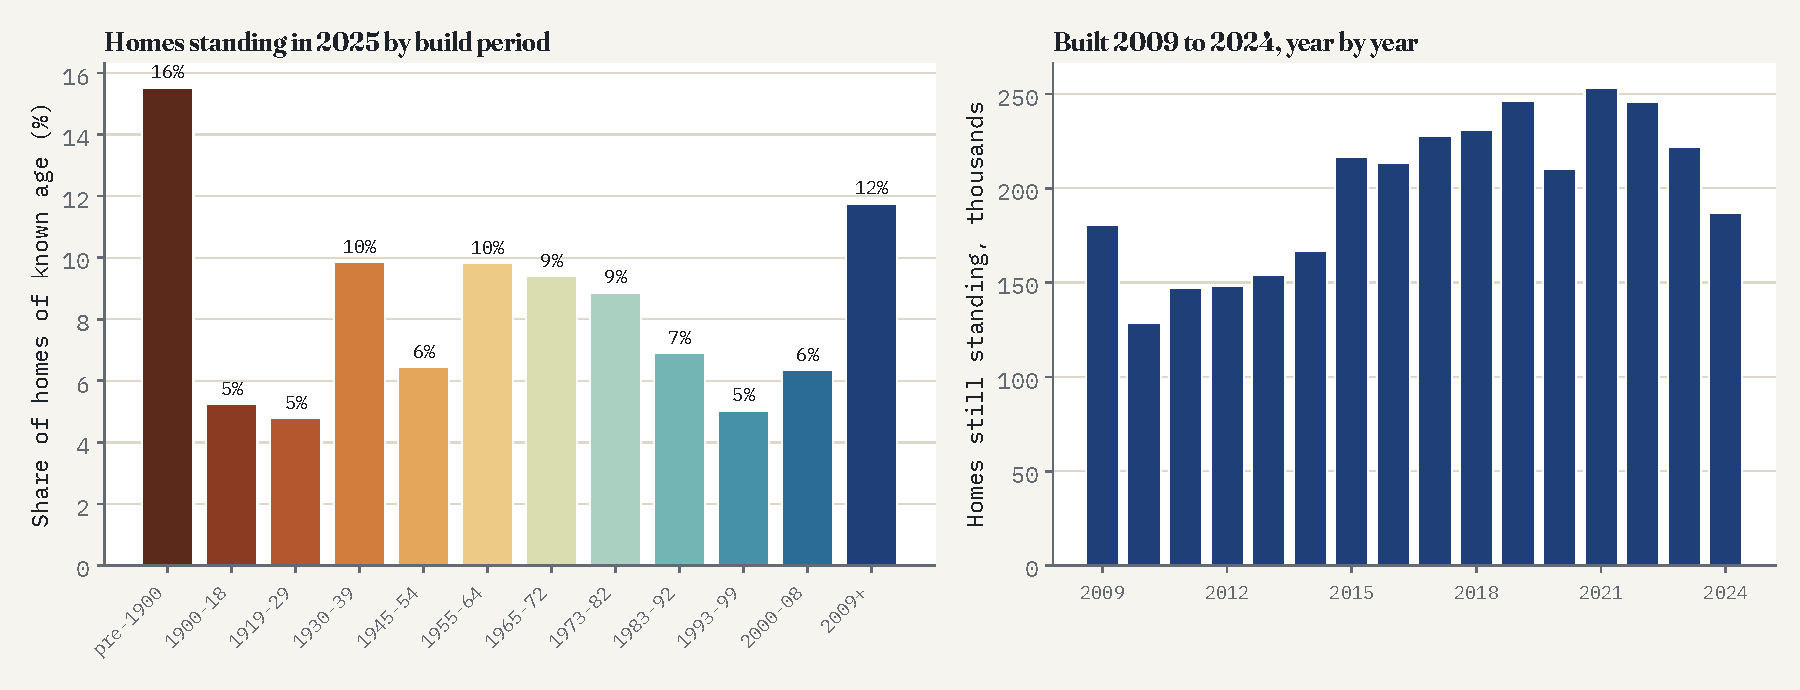
\includegraphics[width=\textwidth]{f_national.pdf}
\caption{Left: homes standing at 31 March 2025 by build period, England and Wales (share of homes of known period). Right: homes standing that were built in each year from 2009 to 2024 (thousands). Source: VOA CTSOP4.1.}\label{fig:national}
\end{figure}

\begin{figure}[tbp]\centering
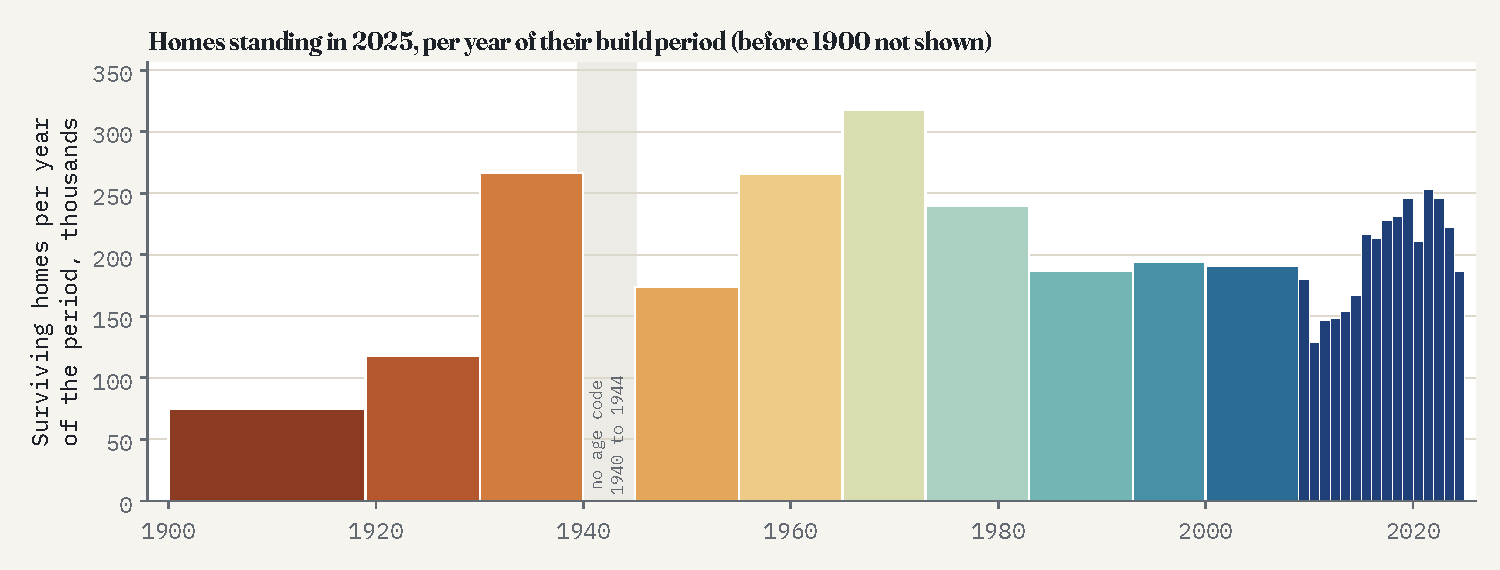
\includegraphics[width=\textwidth]{f_peryear.pdf}
\caption{Surviving homes per year of each build period, England and Wales. Homes built before 1900 are not shown. The grey band marks 1940 to 1944, for which no age code exists.}\label{fig:peryear}
\end{figure}

Table~\ref{tab:regions} gives the same breakdown by region. Wales has an older stock than England: 30.2\% of Welsh homes predate 1919, against 20.2\% in England, and 8.5\% were built from 2009, against 11.9\%. Among English regions, London has the highest pre-1919 share (29.4\%) and the highest interwar share (22.5\%), and the East of England the lowest pre-1919 share (13.7\%). The North East and the West Midlands have the largest post-war shares (30.6\% and 30.3\%), and the East of England, the South East and the South West the largest shares from 1973 to 1999. By mean build year, London is the oldest region (1944) and the East of England the newest (1964).

Figure~\ref{fig:map} maps the median build period of every LSOA. At the LSOA level the median home is post-war (1945 to 1972) in 42.6\% of areas, from 1973 to 1999 in 20.9\%, interwar in 17.5\% and pre-1919 in 13.5\%; in 2.7\% it is from 2000 to 2008 and in 2.8\% from 2009 onwards. In 559 LSOAs at least 90\% of homes predate 1919, and in 227 at least 90\% were built from 2009. The unknown share exceeds 10\% in 138 LSOAs and 50\% in none.

\begin{figure}[tbp]\centering
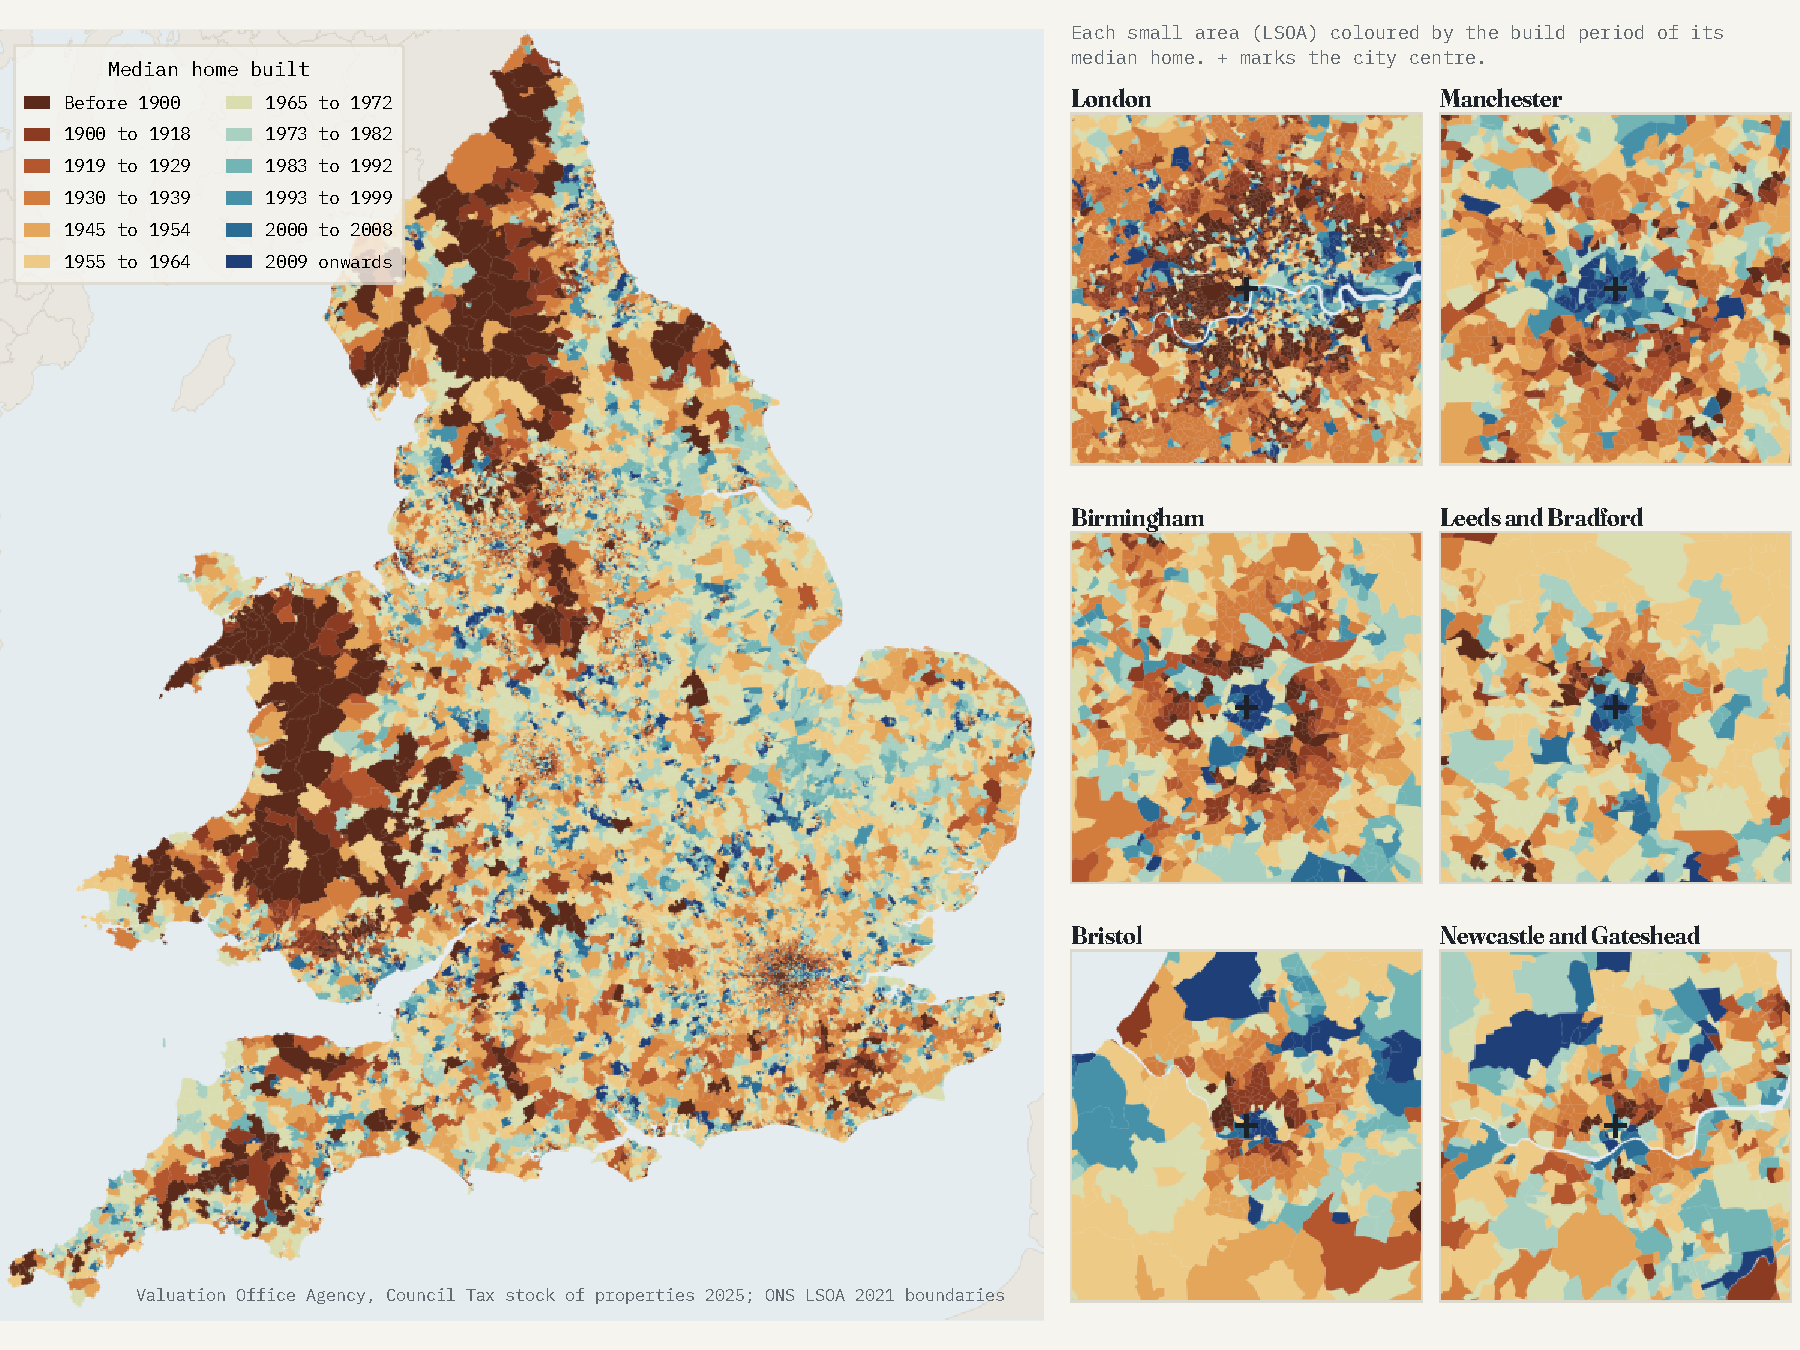
\includegraphics[width=\textwidth]{f_map.pdf}
\caption{Median build period of homes in each of the 35,672 LSOAs of England and Wales, with six city areas at a larger scale (+ marks the centre used in the analysis). Source: VOA CTSOP4.1; ONS LSOA 2021 boundaries.}\label{fig:map}
\end{figure}

\subsection{Local authorities and the new-build frontier}
Table~\ref{tab:la} lists the local authorities with the oldest and newest stock (all 318 are in the released data). Kensington and Chelsea has the highest pre-1919 share, 65.7\%, followed by Hammersmith and Fulham and Haringey; the list mixes inner London boroughs with two Lancashire districts (Pendle and Hyndburn) and three Welsh authorities (Rhondda Cynon Taf, Blaenau Gwent and Gwynedd). The lowest pre-1919 shares are in Basildon (1.1\%), Harlow, Castle Point and Stevenage, three of them districts built around post-war new towns. The highest shares built from 2009 are in Tower Hamlets (31.7\%), South Derbyshire (24.6\%) and Tewkesbury (23.2\%). Figure~\ref{fig:la} places every authority on these two dimensions. Newham is unusual in combining a large pre-1919 stock (37.3\%) with a large recent one (22.8\%).

\begin{table}[tbp]\centering\small\caption{Local authorities with the highest and lowest share of homes built before 1919, and the highest share built from 2009 onwards (shares of homes of known period, \%). Source: VOA CTSOP4.1 (local authority rows).}\label{tab:la}\begin{tabular}{lrrrl}\toprule Local authority & Homes & Before 1919 & 2009 on & Median home\\\midrule
\multicolumn{5}{l}{\textit{Highest share before 1919}}\\
\quad Kensington and Chelsea & 89,250 & 65.7 & 4.1 & Before 1900\\
\quad Hammersmith and Fulham & 95,070 & 55.9 & 12.5 & 1900 to 1918\\
\quad Haringey & 114,960 & 54.1 & 9.0 & 1900 to 1918\\
\quad Pendle & 41,670 & 52.8 & 5.3 & 1900 to 1918\\
\quad Rhondda Cynon Taf & 111,810 & 49.5 & 6.0 & 1919 to 1929\\
\quad Westminster & 132,190 & 49.0 & 9.3 & 1919 to 1929\\
\quad Camden & 113,890 & 48.6 & 9.7 & 1919 to 1929\\
\quad Hyndburn & 37,950 & 47.6 & 4.2 & 1919 to 1929\\
\quad Blaenau Gwent & 33,170 & 46.7 & 4.9 & 1919 to 1929\\
\quad Gwynedd & 62,370 & 46.2 & 6.4 & 1930 to 1939\\
\multicolumn{5}{l}{\textit{Lowest share before 1919}}\\
\quad Basildon & 80,090 & 1.1 & 8.8 & 1973 to 1982\\
\quad Harlow & 40,520 & 1.4 & 13.5 & 1965 to 1972\\
\quad Castle Point & 39,570 & 1.8 & 7.0 & 1965 to 1972\\
\quad Stevenage & 38,430 & 2.0 & 9.0 & 1965 to 1972\\
\quad Crawley & 47,280 & 2.3 & 9.9 & 1973 to 1982\\
\multicolumn{5}{l}{\textit{Highest share from 2009 onwards}}\\
\quad Tower Hamlets & 149,820 & 12.0 & 31.7 & 1993 to 1999\\
\quad South Derbyshire & 51,050 & 15.4 & 24.6 & 1983 to 1992\\
\quad Tewkesbury & 46,250 & 10.4 & 23.2 & 1973 to 1982\\
\quad Newham & 132,600 & 37.3 & 22.8 & 1955 to 1964\\
\quad Vale of White Horse & 64,770 & 11.1 & 22.7 & 1973 to 1982\\
\quad Uttlesford & 40,760 & 19.7 & 22.7 & 1973 to 1982\\
\quad Harborough & 44,900 & 15.3 & 22.6 & 1973 to 1982\\
\quad Milton Keynes & 126,380 & 5.8 & 22.0 & 1983 to 1992\\
\quad Salford & 135,720 & 16.2 & 21.7 & 1965 to 1972\\
\quad South Norfolk & 67,580 & 14.6 & 21.6 & 1973 to 1982\\
\bottomrule\end{tabular}\end{table}

\begin{figure}[tbp]\centering
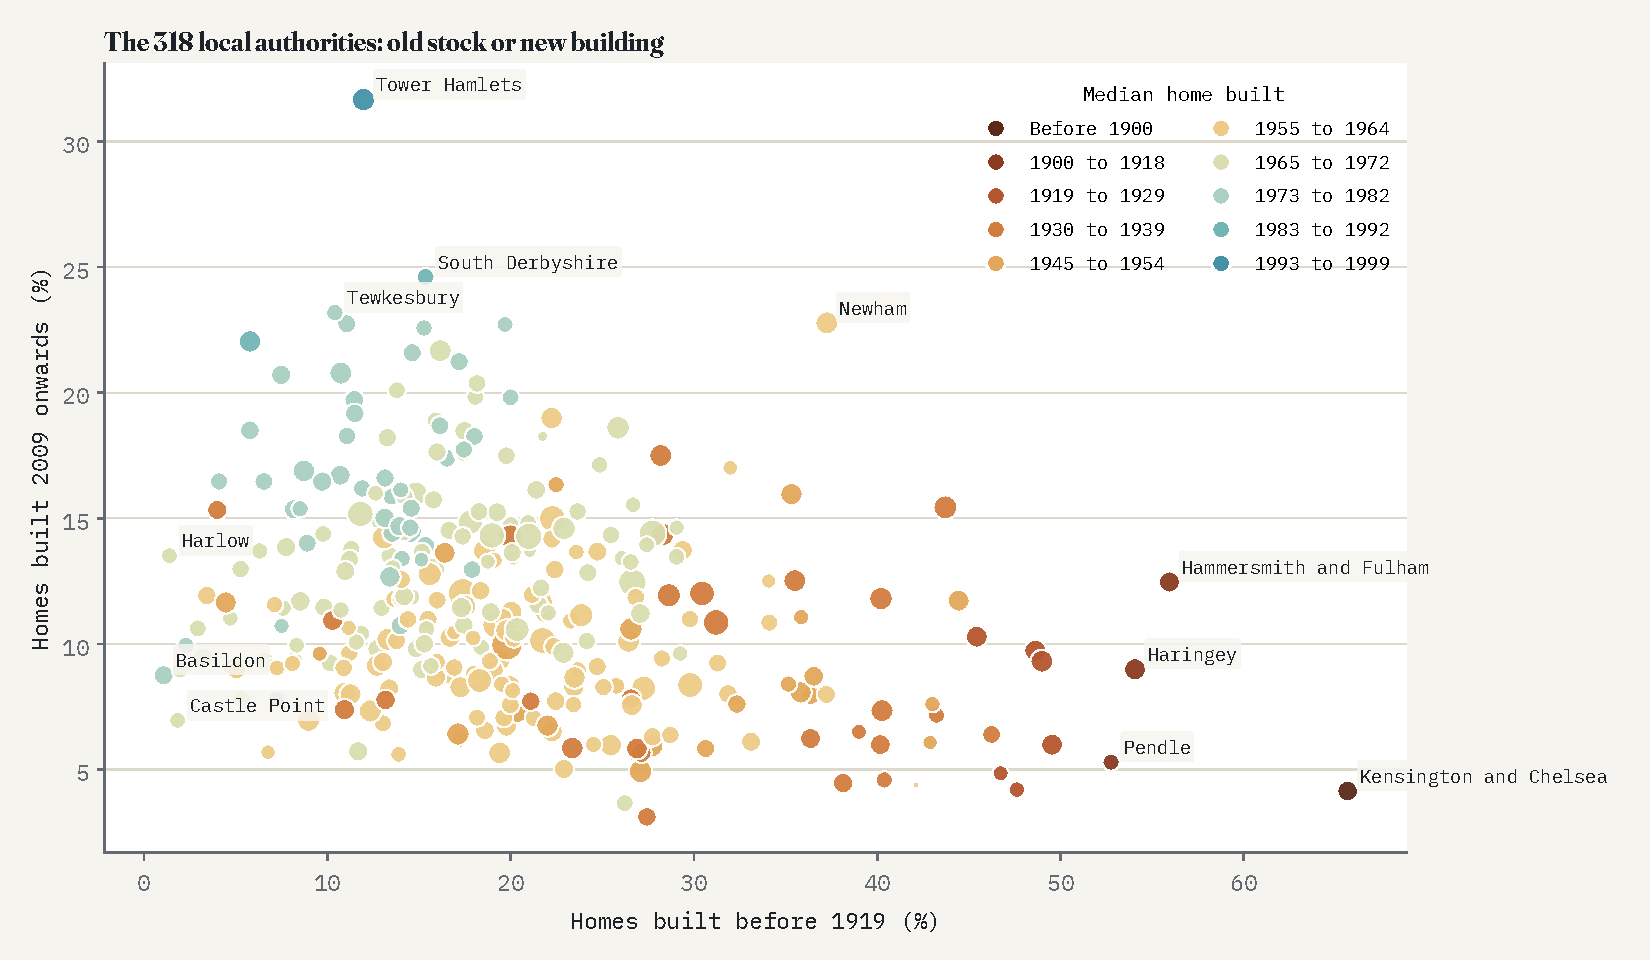
\includegraphics[width=\textwidth]{f_la.pdf}
\caption{Local authorities by share of homes built before 1919 and from 2009 onwards, sized by number of homes and coloured by the build period of the median home.}\label{fig:la}
\end{figure}

In 1,032 LSOAs at least half of the homes of known age were built from 2009 onwards; together they hold 771,470 such homes. They are spread across the country but concentrated in a few authorities: 34 are in Tower Hamlets, 25 in Newham, 21 in Milton Keynes and 20 in Greenwich. By region, 232 are in London and 22 in Wales. New building is spatially concentrated: the tenth of LSOAs with the most homes from 2009 onwards hold 54.7\% of them.

\subsection{Council Tax bands and property types}
In England, the share of a period's homes in the two lowest bands (A and B) and in the three highest (F to H) varies widely (Table~\ref{tab:bands}, Figure~\ref{fig:bands}). Homes built from 1945 to 1954 are the most concentrated in the lowest bands (60.5\% in A or B, 4.1\% in F to H). Homes built before 1900 are polarised: 50.1\% are in A or B but 12.8\% are in F to H, the second highest share of any period after 1993 to 1999 (14.2\%). This is consistent with the VOA's own observation that band A is the most frequent band for the pre-1900, 1900 to 1918, 1919 to 1929, 1945 to 1954 and 1973 to 1982 periods \citep{voa2025com}.

The VOA tables do not cross property type with build period, so types can only be related to the age of areas. Where an LSOA's median home predates 1919, 43\% of its homes are terraced houses and 37\% are flats; where it is interwar, 33\% are semi-detached; where it is from 2009 onwards, 51\% are flats. Across LSOAs weighted by homes, the pre-1919 share correlates with the terraced share at 0.33 and the interwar share with the semi-detached share at 0.39.

\begin{table}[tbp]\centering\small\caption{Council Tax band by build period: share of the period's homes in bands A and B, in the top bands (England F to H; Wales F to I) and the mean band (A = 1). England's bands rest on 1991 values and Wales's on 2003 values, so the two are not comparable.}\label{tab:bands}\begin{tabular}{lrrrrrr}\toprule & \multicolumn{3}{c}{England} & \multicolumn{3}{c}{Wales}\\\cmidrule(lr){2-4}\cmidrule(lr){5-7} Build period & A, B (\%) & F to H (\%) & Mean & A, B (\%) & F to I (\%) & Mean\\\midrule
Before 1900 & 50.1 & 12.8 & 2.94 & 45.8 & 11.8 & 3.11\\
1900 to 1918 & 52.3 & 9.4 & 2.77 & 49.3 & 8.0 & 2.91\\
1919 to 1929 & 49.1 & 8.6 & 2.82 & 41.3 & 10.6 & 3.19\\
1930 to 1939 & 38.7 & 8.8 & 3.14 & 24.9 & 15.9 & 3.72\\
1945 to 1954 & 60.5 & 4.1 & 2.36 & 53.7 & 6.0 & 2.68\\
1955 to 1964 & 41.1 & 6.8 & 2.93 & 39.8 & 9.2 & 3.12\\
1965 to 1972 & 43.4 & 6.0 & 2.85 & 31.1 & 9.3 & 3.36\\
1973 to 1982 & 48.2 & 6.8 & 2.79 & 32.2 & 12.4 & 3.43\\
1983 to 1992 & 39.9 & 10.0 & 3.16 & 26.4 & 17.2 & 3.75\\
1993 to 1999 & 31.4 & 14.2 & 3.53 & 19.9 & 19.7 & 3.95\\
2000 to 2008 & 32.1 & 12.0 & 3.42 & 9.7 & 27.9 & 4.56\\
2009 onwards & 33.1 & 11.0 & 3.35 & 20.7 & 18.9 & 3.92\\
\bottomrule\end{tabular}\end{table}

\begin{figure}[tbp]\centering
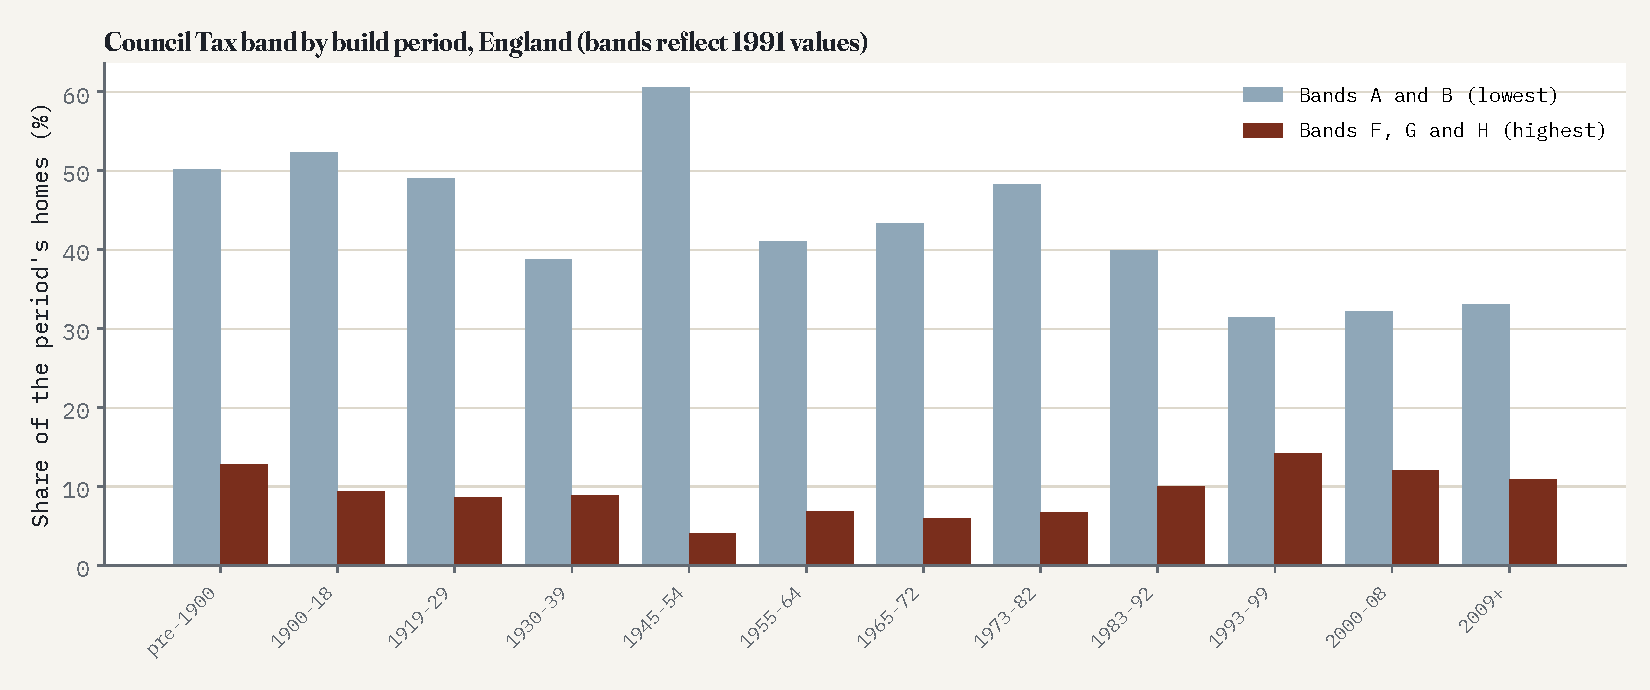
\includegraphics[width=\textwidth]{f_bands.pdf}
\caption{Share of each build period's homes in Council Tax bands A and B and in bands F to H, England (bands based on 1991 values).}\label{fig:bands}
\end{figure}

\subsection{Rings of age in the cities}
The catchments of the 34 cities contain 20,837 LSOAs and 15,642,230 homes of known age, in 244 local authorities. Figure~\ref{fig:rings} pools them by 1 km distance band. Two features stand out. Pre-1919 homes peak not at the centre but 1 to 2 km out, where they make up 40.1\% of homes. And recent building is the largest group in the first kilometre: 32.2\% of its homes were built from 2009 and 15.1\% from 2000 to 2008. Beyond about 3 km the profile is flatter: the interwar share peaks 3 to 4 km out (22.8\%), and from 3 km outward post-war homes are the largest group. Figure~\ref{fig:cities} shows the same profiles for six cities.

\begin{figure}[tbp]\centering
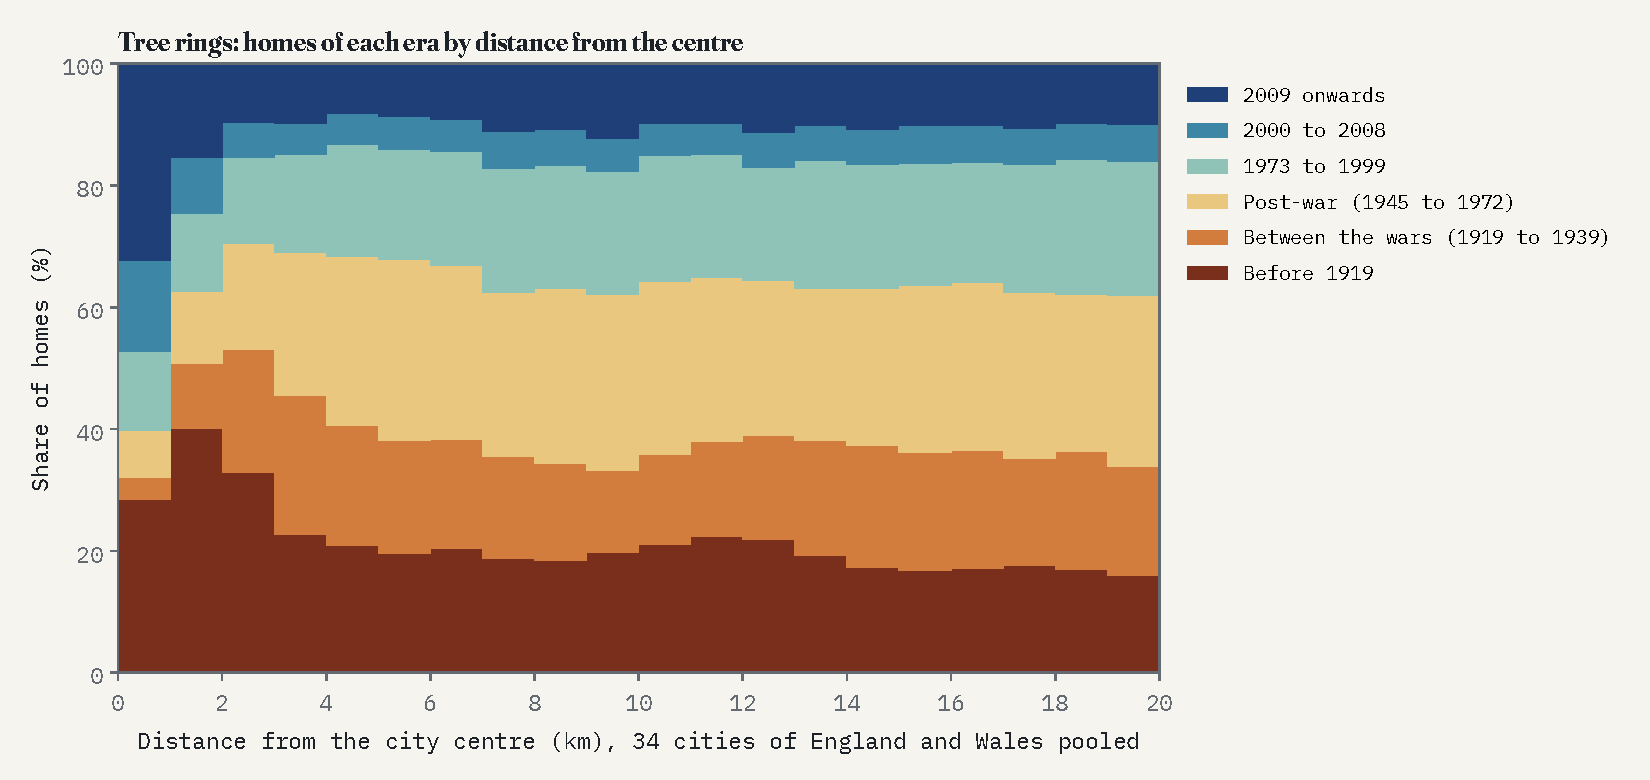
\includegraphics[width=\textwidth]{f_rings.pdf}
\caption{Share of homes by build era in 1 km distance bands from the centre, 34 cities pooled (20,837 LSOAs within 20 km of a centre).}\label{fig:rings}
\end{figure}

\begin{figure}[tbp]\centering
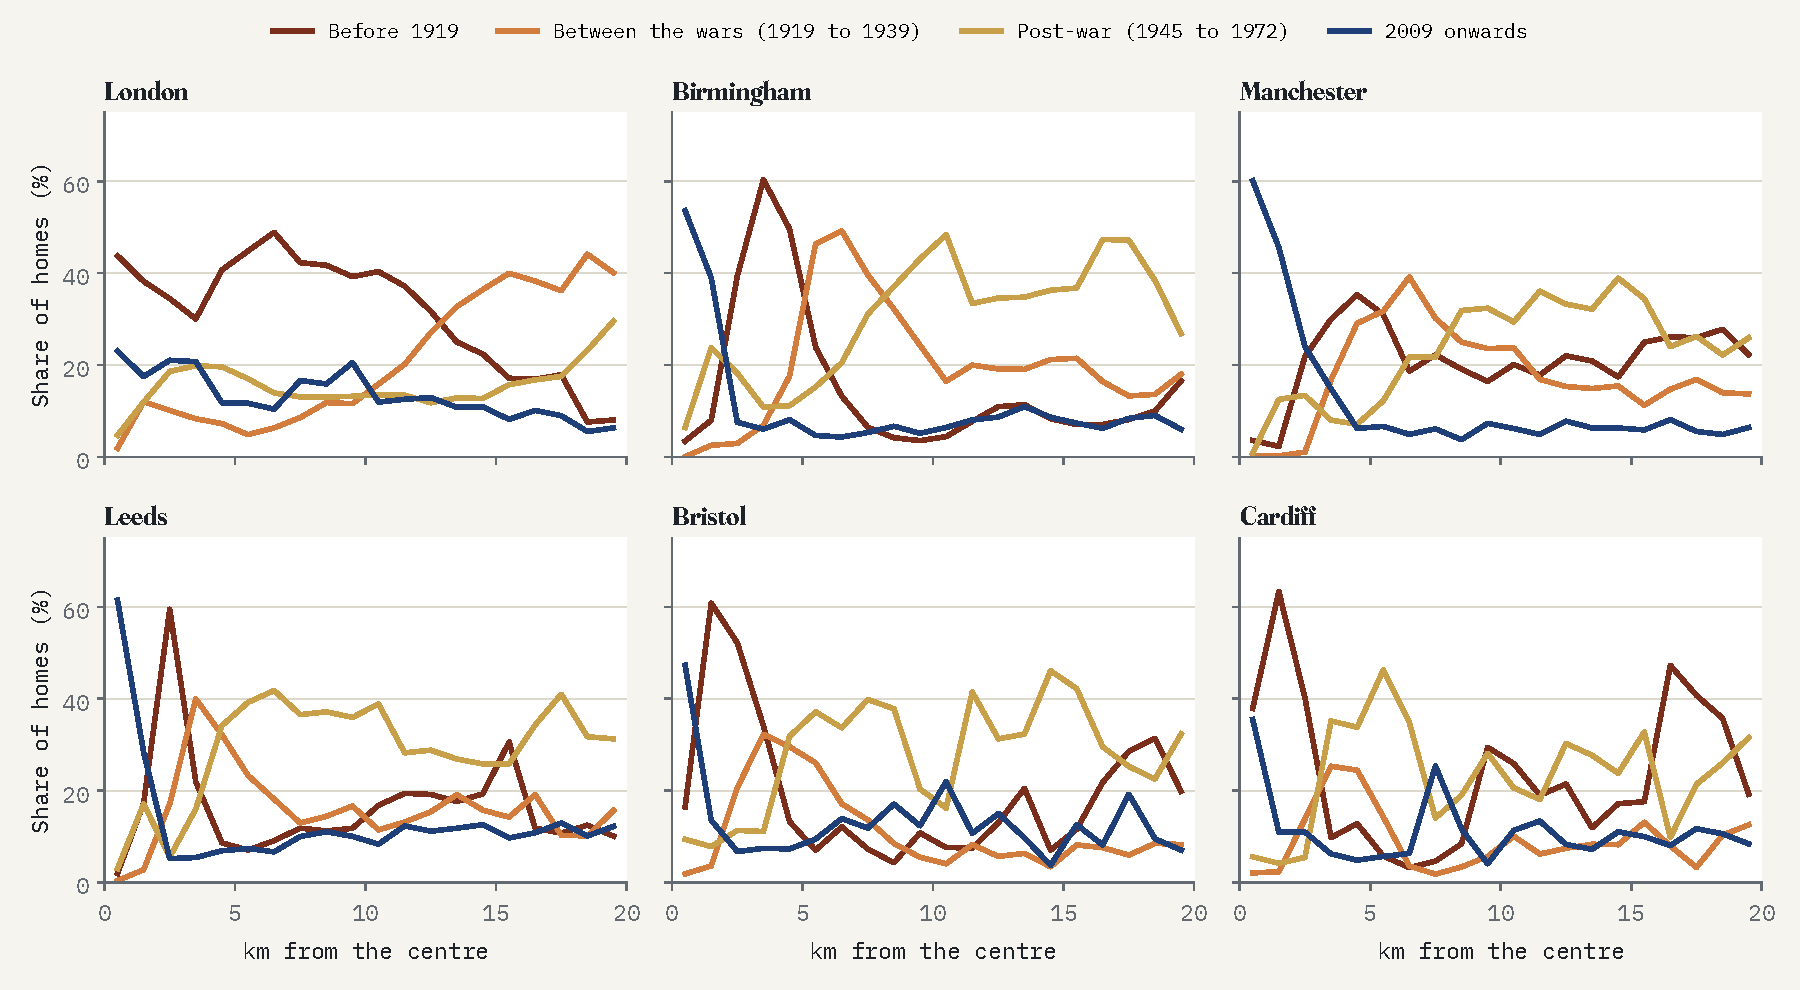
\includegraphics[width=\textwidth]{f_cities.pdf}
\caption{Share of homes of four eras by distance from the centre in six cities (1 km bands with at least 1,000 homes of known age).}\label{fig:cities}
\end{figure}

\paragraph{H1.} Model M1 gives a positive slope: the mean build year rises by 0.61 years per kilometre from the centre (95\% CI 0.36 to 0.85; $N=20,837$ LSOAs, 244 local authority clusters). By the plan's criterion this would support H1. But the placebo test (Section~\ref{sec:robust}) shows that a slope of this size arises easily without real centres: with centres moved 10 km in a random direction the slope is at least as steep in 8.5\% of 200 draws, and the real slope (0.61) is below the placebo 95th percentile (0.63). By the rule set in advance, the linear gradient is not evidence of a centre-specific structure. Figure~\ref{fig:bins} shows why: relative to the first kilometre, LSOAs 1 to 3 km out are on average 22.1 to 22.5 years older, and the mean year then rises slowly, so a single line is a poor description of a profile that is youngest at the centre, oldest just outside it and rises gently beyond. The quadratic check (R9) points the same way.

\paragraph{H2.} The ring structure, by contrast, is strong. In Model M2, each successive period from before 1900 to 1965 to 1972 stands on average 4.3\% farther from the centre (coefficient 0.042 in logs, 95\% CI 0.031 to 0.054; 238 city-period cells, 34 clusters). The Spearman correlation between period order and mean distance is positive in 33 of 34 cities, with a median of 0.46. Figure~\ref{fig:cohort} shows the full profile over all twelve periods, relative to each city's mean distance of all homes. The closest period is 1900 to 1918 (mean relative distance 0.81), not before 1900 (0.94), plausibly because the pre-1900 stock includes the cores of the older towns and villages that lie within the catchments. The interwar periods stand at 0.89 and 0.86, the post-war periods at 1.03 to 1.11, and the late twentieth century at 1.09 to 1.12.

\paragraph{H3.} Then the order reverses. Homes built from 2000 to 2008 stand 8.9\% closer to the centre than homes of 1983 to 1992, and homes from 2009 onwards 8.1\% closer, while homes of 1993 to 1999 stand 2.3\% farther out. The pre-specified statistic M3 gives a mean log difference between the 2009 onwards and 1983 to 1999 cohorts of $-$0.095 (95\% CI $-$0.139 to $-$0.050), that is, homes from 2009 onwards stand 9.0\% closer to the centre; the difference is negative in 26 of 34 cities. H3 is supported.

\paragraph{H4.} In 32 of 34 cities the band with the highest interwar share lies strictly between the band with the highest pre-1919 share and the band with the highest 1955 to 1972 share (median peak bands 1, 3 and 6.5 km, counting bands by their inner edge). Table~\ref{tab:citylist} gives the peaks for every city.

\subsection{Individual cities}
The pooled estimates hide differences between cities that the appendix tables make visible (Table~\ref{tab:citylist}). London is the one city in which the H2 ordering fails: its Spearman correlation is $-$0.11. This is mostly a matter of scale. A 20 km circle around Charing Cross covers inner and much of outer London but cuts through its interwar suburbs, which dominate several outer boroughs (Harrow, Barking and Dagenham, Bexley and Sutton have the highest interwar shares of any local authority, from 40.8\% to 51.8\%). London's peak interwar band lies 18 km from the centre, beside its peak band for 1955 to 1972, so the H4 order also fails there; the other city where it fails is Exeter, a small city whose interwar and post-war peaks fall in the same band. With London excluded, all estimates are essentially unchanged (Section~\ref{sec:robust}), so London neither drives nor contradicts the pooled result.

The reversal measured by M3 is strongest in Manchester, where homes built from 2009 stand 34.7\% closer to the centre than those of 1983 to 1999, and is also large in the other big regional centres (Table~\ref{tab:citylist}). It goes the other way in eight cities (Blackpool, Ipswich, Oxford, Portsmouth, Southend-on-Sea, Stoke-on-Trent, Sunderland and York), none of them among the five largest, where the newest homes stand farther out than those of 1983 to 1999. Recentralisation of new housing is therefore a feature of most, not all, cities, and of the largest ones most clearly.

\begin{table}[tbp]\centering\small\caption{Main pre-specified estimates. M1: weighted least squares of LSOA mean build year on distance (km) with city fixed effects, weights = homes of known period, SE clustered by local authority. M2: OLS of log mean distance of each period's homes on period order (before 1900 = 0 to 1965 to 1972 = 6), city fixed effects, SE clustered by city. M3: mean over cities of the log difference in mean distance between homes built 2009 onwards and 1983 to 1999, $t$ interval. Placebo: centres moved 10 km in a random direction, 200 draws.}\label{tab:models}\setlength{\tabcolsep}{4pt}\begin{tabular}{lrrrl}\toprule Model & Estimate & 95\% CI & $N$ & Placebo p95\\\midrule
M1 (years per km) & 0.605 & [0.362, 0.848] & 20,837 LSOAs, 244 clusters & 0.635 (fails)\\
\quad clustered by city & & [0.336, 0.874] & 34 clusters & \\
M2 (log distance per period) & 0.042 & [0.031, 0.054] & 238 cells, 34 clusters & 0.010 (passes)\\
\quad cities with positive Spearman $\rho$ & 33 of 34 & & & \\
M3 (log difference) & $-$0.095 & [$-$0.139, $-$0.050] & 34 cities & \\
\quad cities with a negative difference & 26 of 34 & & & \\
M1 quadratic: distance & 1.936 & & & \\
\quad distance squared & $-$0.065 & $p$ = 0.030 & & \\
\bottomrule\end{tabular}\end{table}

\begin{figure}[tbp]\centering
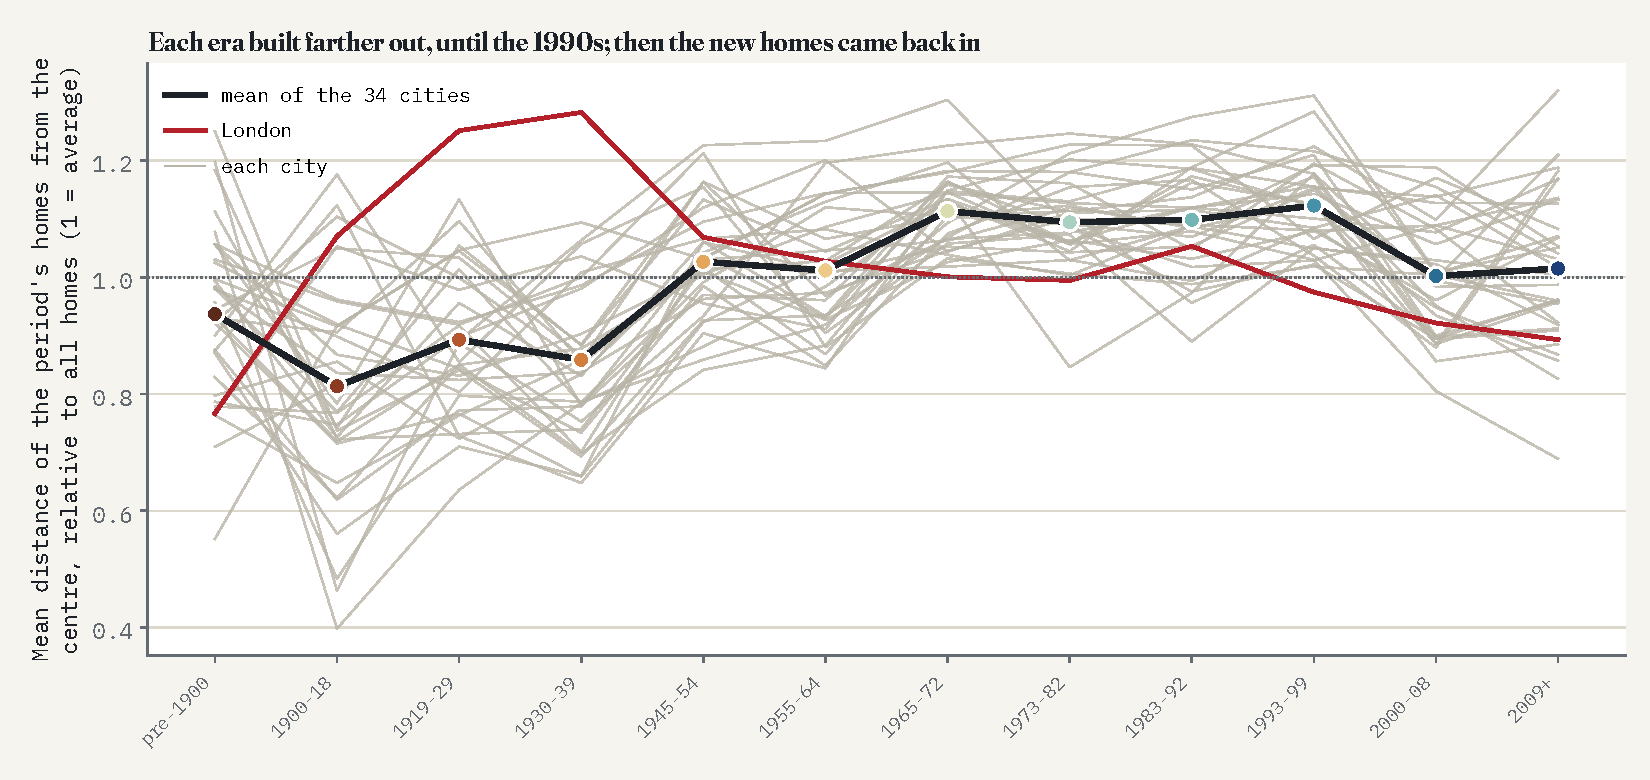
\includegraphics[width=\textwidth]{f_cohort.pdf}
\caption{Mean distance from the centre of each period's homes, relative to the mean distance of all homes in the catchment (1 = average), for each city (grey), London (red) and the mean of the 34 cities (black, points coloured by period).}\label{fig:cohort}
\end{figure}

\begin{figure}[tbp]\centering
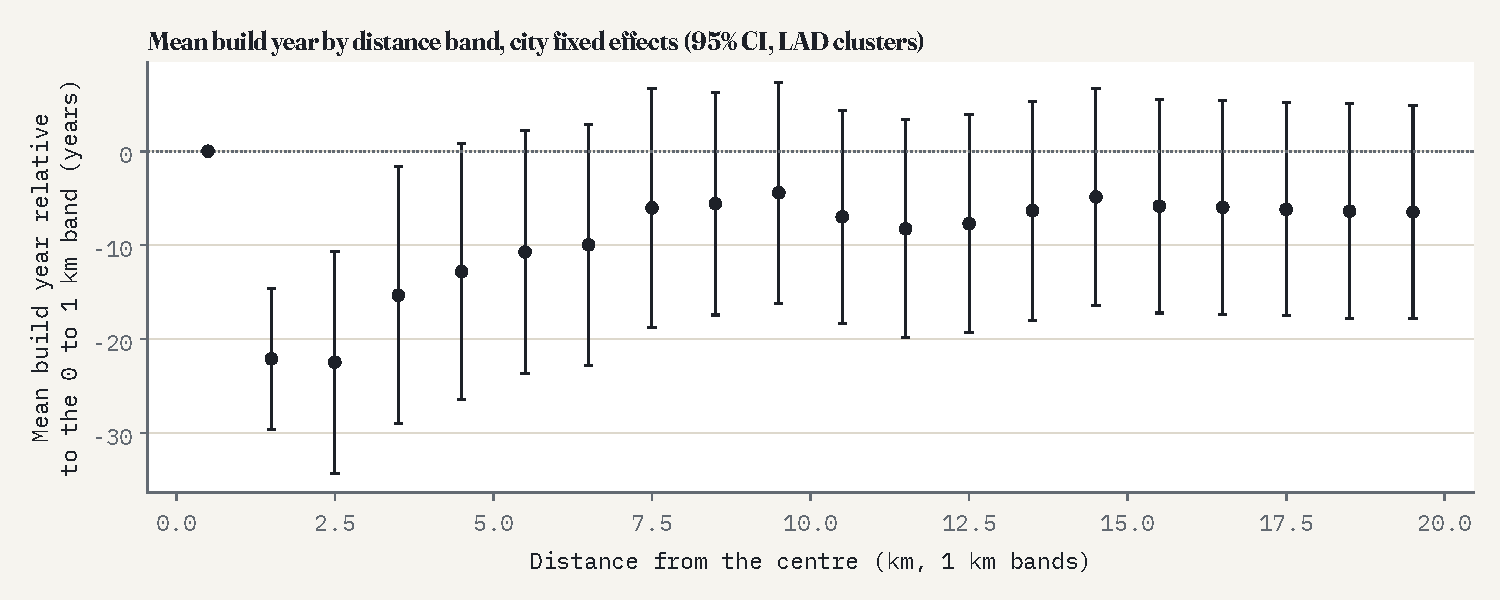
\includegraphics[width=0.92\textwidth]{f_bins.pdf}
\caption{Model M1 with 1 km distance bins: mean build year relative to the first kilometre, with city fixed effects, weighted by homes of known age; 95\% intervals with standard errors clustered by local authority.}\label{fig:bins}
\end{figure}

\section{Robustness}
\label{sec:robust}
Table~\ref{tab:robust} and Figure~\ref{fig:robust} report all planned checks. None changes the sign or the conclusion for H2 or H3.

\paragraph{Measurement (R1, R2, R7).} Counting suppressed cells as 2.5 gives an M2 coefficient of 0.042 and an M3 difference of $-$0.079. The pre-1900 midpoint affects only M1, whose slope is 0.77 with a midpoint of 1850 and 0.51 with 1890. Restricting to LSOAs with less than 2\% of homes of unknown age (19,133 LSOAs) gives 0.043 and $-$0.093.

\paragraph{Catchment and centres (R3, R4).} With 10 km catchments the gradients are steeper (M2 0.090, M3 $-$0.183), and with 30 km flatter but still clear (M2 0.021, 95\% CI 0.010 to 0.032; M3 $-$0.057, CI $-$0.097 to $-$0.017), as expected when the catchment includes more towns that are not part of the city. With Natural Earth's centres, M2 is 0.041 and M3 $-$0.082.

\paragraph{Regions and London (R5).} Leaving out each region in turn, M2 ranges from 0.037 to 0.043 and M3 from $-$0.106 to $-$0.071, and every interval excludes zero. Without London, M2 is 0.042 and M3 $-$0.090.

\paragraph{Placebo (R6).} With every centre moved 10 km in a random direction (200 draws), the M2 coefficient has a mean of 0.005, a 95th percentile of 0.010 and a maximum of 0.014, against 0.042 with the real centres: no draw comes close. The M1 slope, by contrast, has a placebo mean of 0.29, a 95th percentile of 0.63 and a maximum of 0.88, so the real slope of 0.61 is not unusual. The ordering of the periods' homes around a centre is specific to real centres; the linear rise of mean build year with distance is not.

\paragraph{Inference and scale (R8, R9).} Clustering M1 by city instead of local authority gives a 95\% interval of 0.34 to 0.87. At MSOA level (4,210 MSOAs), M1 is 0.62 years per km and M2 0.041, close to the LSOA results. A quadratic in distance gives a negative squared term ($p=0.030$) with a turning point at 14.9 km, consistent with the flattening in Figure~\ref{fig:bins}.

\begin{table}[tbp]\centering\footnotesize\setlength{\tabcolsep}{4pt}\caption{Planned robustness checks: estimates and 95\% intervals for M1 (years per km), M2 (log distance per period) and M3 (log difference, 2009 onwards against 1983 to 1999). R8 MSOA: M1 with SE clustered by city.}\label{tab:robust}\begin{tabular}{lrlll}\toprule Check & LSOAs & M1 & M2 & M3\\\midrule
Main specification & 20,837 & 0.61 [0.36, 0.85] & 0.042 [0.031, 0.054] & $-$0.095 [$-$0.139, $-$0.050]\\
R1 suppressed cells = 2.5 & 20,837 & 0.62 [0.38, 0.86] & 0.042 [0.030, 0.053] & $-$0.079 [$-$0.119, $-$0.039]\\
R2 pre-1900 midpoint 1850 & 20,837 & 0.77 [0.48, 1.05] & 0.042 [0.031, 0.054] & $-$0.095 [$-$0.139, $-$0.050]\\
R2 pre-1900 midpoint 1890 & 20,837 & 0.51 [0.29, 0.73] & 0.042 [0.031, 0.054] & $-$0.095 [$-$0.139, $-$0.050]\\
R3 catchment 10 km & 11,047 & 1.73 [0.74, 2.72] & 0.090 [0.077, 0.102] & $-$0.183 [$-$0.252, $-$0.114]\\
R3 catchment 30 km & 28,290 & 0.37 [0.22, 0.51] & 0.021 [0.010, 0.032] & $-$0.057 [$-$0.097, $-$0.017]\\
R4 Natural Earth centres & 20,989 & 0.61 [0.37, 0.86] & 0.041 [0.029, 0.054] & $-$0.082 [$-$0.122, $-$0.042]\\
R5 without London & 16,349 & 0.59 [0.36, 0.81] & 0.042 [0.030, 0.053] & $-$0.090 [$-$0.136, $-$0.045]\\
R7 unknown share below 2\% & 19,133 & 0.67 [0.42, 0.91] & 0.043 [0.030, 0.056] & $-$0.093 [$-$0.138, $-$0.049]\\
\midrule\multicolumn{5}{l}{\textit{R5 leaving out one region}}\\
\quad without North East & 19,468 & 0.61 [0.35, 0.86] & 0.043 [0.030, 0.055] & $-$0.099 [$-$0.145, $-$0.053]\\
\quad without North West & 17,998 & 0.68 [0.44, 0.93] & 0.039 [0.027, 0.050] & $-$0.088 [$-$0.127, $-$0.049]\\
\quad without Yorkshire and the Humber & 18,433 & 0.66 [0.39, 0.93] & 0.041 [0.028, 0.054] & $-$0.083 [$-$0.129, $-$0.036]\\
\quad without East Midlands & 19,508 & 0.61 [0.36, 0.87] & 0.043 [0.031, 0.056] & $-$0.096 [$-$0.144, $-$0.048]\\
\quad without West Midlands & 18,499 & 0.58 [0.31, 0.85] & 0.040 [0.028, 0.052] & $-$0.087 [$-$0.132, $-$0.042]\\
\quad without East of England & 19,002 & 0.58 [0.31, 0.85] & 0.037 [0.024, 0.051] & $-$0.095 [$-$0.143, $-$0.048]\\
\quad without London & 16,349 & 0.59 [0.36, 0.81] & 0.042 [0.030, 0.053] & $-$0.090 [$-$0.136, $-$0.045]\\
\quad without South East & 18,736 & 0.51 [0.26, 0.77] & 0.039 [0.024, 0.054] & $-$0.106 [$-$0.153, $-$0.058]\\
\quad without South West & 19,487 & 0.60 [0.35, 0.85] & 0.037 [0.026, 0.049] & $-$0.071 [$-$0.114, $-$0.028]\\
\quad without Wales & 20,053 & 0.62 [0.37, 0.88] & 0.043 [0.031, 0.055] & $-$0.096 [$-$0.142, $-$0.050]\\
\midrule R8 MSOA level & 4,210 MSOAs & 0.62 [0.36, 0.89] & 0.041 & \\
R6 placebo centres, mean (95th pct) & 200 draws & 0.29 (0.63) & 0.005 (0.010) & \\
\bottomrule\end{tabular}\end{table}

\begin{figure}[tbp]\centering
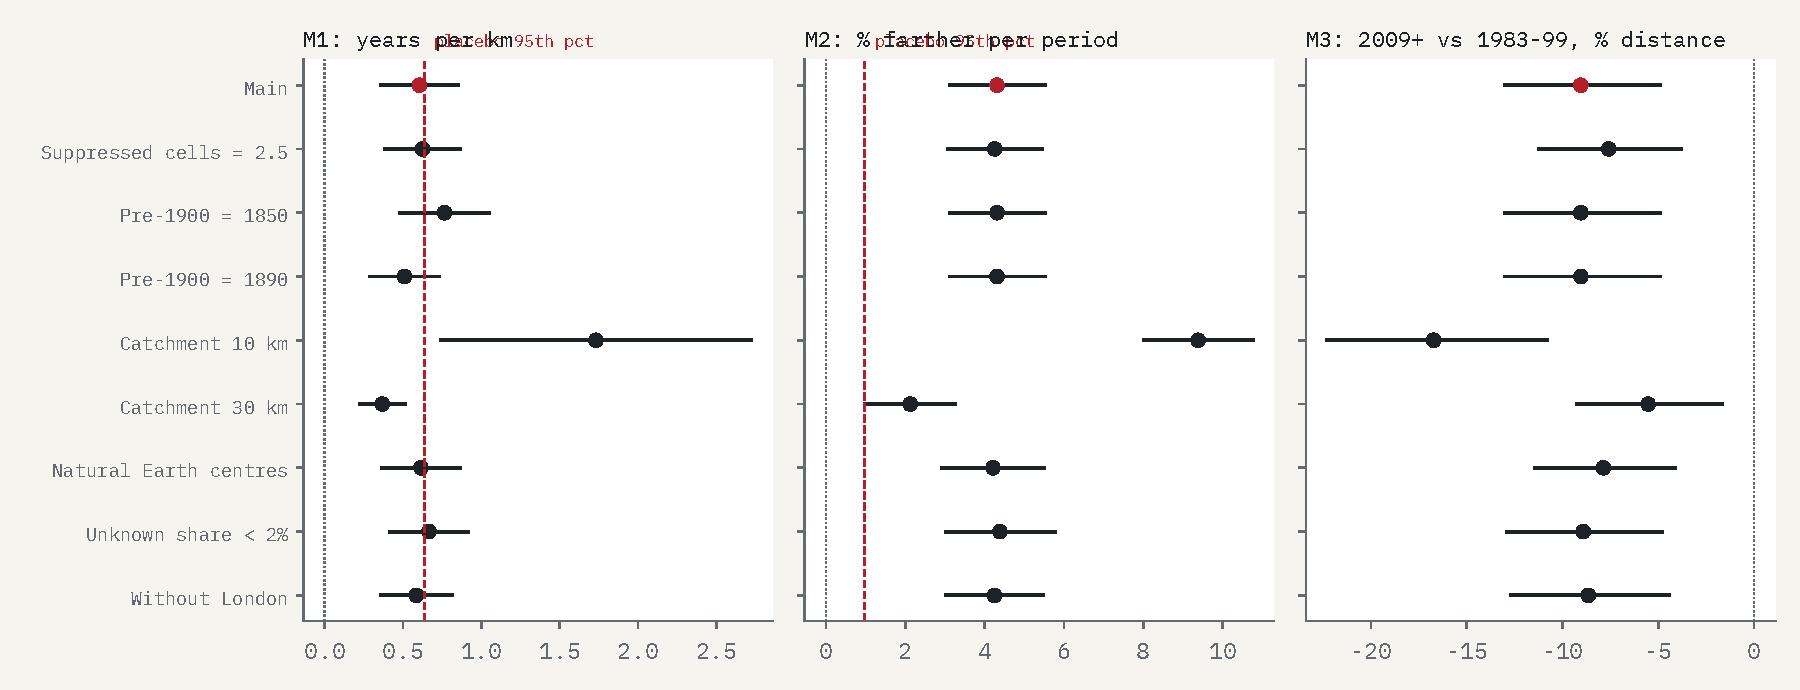
\includegraphics[width=\textwidth]{f_robust.pdf}
\caption{Main estimates and planned robustness checks for M1, M2 (as \% per period) and M3 (as \%), with 95\% intervals. Dashed red lines: 95th percentile of the placebo estimates with centres moved 10 km at random (200 draws).}\label{fig:robust}
\end{figure}

\paragraph{Exploratory: band and age within local authorities.} Not in the plan, I regressed the mean Council Tax band of English LSOAs (A = 1 to H = 8) on their mean build year and property type shares with local authority fixed effects. Holding the type mix fixed, an LSOA whose homes are a decade newer on average has a mean band $-$0.022 lower (95\% CI $-$0.032 to $-$0.012; 33,755 LSOAs, 296 clusters). The association is small and is reported only as a description.

\section{Discussion}
\label{sec:discussion}
\subsection{Rings, but not a gradient}
The housing stock of English and Welsh cities is ordered in rings of age much as vintage models predict. Through the twentieth century, each period's homes were built, and survive, farther from the centre than the last, and the interwar homes sit between the Victorian and Edwardian ring and the post-war periphery in almost every city. That this ordering is specific to the real centres, and not a by-product of the general spatial pattern of building, is shown by the placebo test.

The simplest version of the prediction, that average age falls steadily with distance, does not hold in a useful sense. The centre is not the oldest place in the city: the oldest ring lies one to two kilometres out, and the centre itself is now among the youngest. This is the pattern that models with redevelopment predict once the oldest central housing has been replaced \citep{wheaton1982,braid2001}, and that \citet{brueckner2009} discuss as a route to the return of richer households to central areas. The data cannot say whether the central housing replaced older homes, offices, warehouses or industrial land; the conversion of commercial land to housing is one documented route to recentralisation elsewhere \citep{xu2023}.

\subsection{Recentralisation}
The reversal after the 1990s is the most policy-relevant finding. Homes built from 2009 stand closer to city centres than those built from 1983 to 1999 in 26 of the 34 cities, and the first kilometre around the centres, where 79\% of homes are flats, is led by homes built since 2000 (32\% from 2009 onwards and 15\% from 2000 to 2008). The pattern is consistent with a shift of new building towards central and previously developed land, the aim of brownfield-first policy \citep{wong2010} and of the residential revival of city centres \citep{bromley2005}. It is not evidence about any particular policy, and the size of the shift, about 9\% in mean distance, is modest: most new homes are still built well away from the centres, and the post-2009 cohort is on average about as far out as the stock as a whole.

\subsection{What the map adds}
For research, the LSOA tables offer a complete and annually updated measure of building age that can be joined to any small-area data set built on 2021 geographies. Studies of neighbourhood change in the tradition of \citet{rosenthal2008} and \citet{brueckner2009} need a measure of the age of the stock, and the VOA counts provide one for England and Wales at a scale fine enough to separate a terrace from the estate behind it. The city profiles released with this paper (the mean distance of each period's homes and the share of each era by distance band) can be used as a simple description of urban form against which models of growth and redevelopment can be checked \citep{harrison1974,wheaton1982,hanlon2022}.

For policy, the age of the stock matters wherever the rules or the costs differ by age: maintenance and adaptation, the treatment of older and historic buildings \citep{waights2019}, and the measurement of how much new housing is being built and where. The new-build frontier identified here is concentrated in a small number of places: a tenth of LSOAs hold 55\% of the homes built since 2009. The interactive map lets any reader look up the profile of a neighbourhood and compare it with the national figures.

\subsection{Rings and the assumptions of vintage models}
Vintage models make strong simplifying assumptions: a single centre, growth only at the edge, and either no redevelopment or redevelopment only when the old structure is worth less than the land under it \citep{brueckner1980,wheaton1982}. The cities of England and Wales depart from each of these, and the results show where. Growth at the edge is the dominant pattern through the twentieth century, which is why the rings appear so clearly in M2. But the edge is not a clean line: many LSOAs contain homes from several periods, the pre-1900 stock is scattered through the catchments in older settlements, and growth has leapt over land that was filled in later \citep{rodriguez1986}. The recent return of building to the centre is the departure that the simplest models do not anticipate and that models with redevelopment do \citep{braid2001}. Read this way, the stock of 2025 is a record of a century of outward growth on which a period of inward redevelopment has begun to be written.

\subsection{Limitations}
\paragraph{Survival.} The VOA counts homes standing in 2025. Homes demolished before then, through redevelopment, clearance \citep{yelling2000} or war damage, are absent, and homes converted into several flats may appear as more than one property. The age profile of an area is therefore the outcome of building and of replacement. This matters most for inner areas, where the absence of very old homes at the centre may reflect demolition rather than late development. The data cannot separate the two.

\paragraph{The age code.} The build period is the VOA's age code, an administrative assessment rather than a survey of construction dates. The pre-1900 class is open-ended and covers several centuries; the periods are of unequal length; there is no code for 1940 to 1944; and recent single years may be incomplete if newly built homes enter the lists with a lag. Less than 1\% of homes have no code, but the share is higher in some places (South Holland: 5.9\%).

\paragraph{Geography.} The analysis uses one centre per city, a straight-line distance and a fixed 20 km catchment. Polycentric conurbations such as the West Midlands, Greater Manchester or West Yorkshire are imperfectly described by distance to the nearest of a few centres, and the catchments include free-standing towns. LSOAs vary in area, and the representative point of a large rural LSOA can be far from its homes. The robustness checks vary each of these choices, but none replaces a full model of urban form.

\paragraph{Survival and the inner city.} The finding that the first kilometre is now young could arise in two ways that the data cannot tell apart: the centres may always have had few homes, with recent building on land that was never residential, or older central homes may have been replaced. Either way, the result describes the stock that people live in now, which is what matters for most uses of the map. It is not a history of building, and it should not be read as evidence that any period built more or fewer homes in a place than survive there today. The same caution applies to the rings: a ring of surviving pre-1919 housing 1 to 2 km from the centre is consistent with an older ring further in having been replaced, as models with redevelopment predict \citep{wheaton1982}, but it does not show it.

\paragraph{Inference.} The city-level tests treat 34 cities as independent units; cities in the same conurbation share history. The models are descriptive. They say where the homes of each period stand, not why.

\section{Conclusion}
\label{sec:conclusion}
Using a complete administrative count of the Council Tax stock at 31 March 2025, this paper maps the age of the housing stock in all 35,672 small areas of England and Wales and tests four pre-specified hypotheses about its spatial order in 34 cities. About a fifth of homes predate 1919 and a quarter date from 1945 to 1972. Within cities, the homes of each twentieth-century period stand farther from the centre than those of the period before, a pattern specific to real centres; the interwar ring sits between the pre-1919 core and the post-war periphery in 32 of 34 cities; and since 2000 the direction has reversed, with the newest homes standing closer in and forming the largest group of homes in the first kilometre around the centres. A single linear gradient in average age is not a good description of this structure. The data, maps and code are released for reuse.

\section*{Data availability statement}
Data and code: Zenodo DOI https://doi.org/10.5281/zenodo.24113860. The interactive map is at \url{https://maps.tristanhotham.com/house-age/} and the repository at \url{https://github.com/Tristan-Hotham/house-age}. The repository holds the derived LSOA, MSOA and local authority tables, the city list, the city profiles, the model outputs and the code. The VOA tables are Official Statistics under the Open Government Licence v3.0; the LSOA boundaries are ONS data under the Open Government Licence v3.0 (contains OS data, Crown copyright and database right).

\section*{AI statement}
I wrote the text, with drafting and editing assistance from Claude (Anthropic), which also helped prepare the analysis code. I reviewed and checked all text and results.

\begin{thebibliography}{99}\small
\bibitem[Arnott et al.(1999)]{arnott1999} Arnott, R., Braid, R., Davidson, R. and Pines, D. (1999) A general equilibrium spatial model of housing quality and quantity. \textit{Regional Science and Urban Economics} 29(3), 283 to 316.
\bibitem[Boughton(2018)]{boughton2018} Boughton, J. (2018) \textit{Municipal Dreams: The Rise and Fall of Council Housing}. London: Verso.
\bibitem[Braid(2001)]{braid2001} Braid, R. M. (2001) Spatial growth and redevelopment with perfect foresight and durable housing. \textit{Journal of Urban Economics} 49(3), 425 to 452.
\bibitem[Bromley et al.(2005)]{bromley2005} Bromley, R. D. F., Tallon, A. R. and Thomas, C. J. (2005) City centre regeneration through residential development: contributing to sustainability. \textit{Urban Studies} 42(13), 2407 to 2429. doi:10.1080/00420980500379537.
\bibitem[Brueckner(1980)]{brueckner1980} Brueckner, J. K. (1980) A vintage model of urban growth. \textit{Journal of Urban Economics} 8(3), 389 to 402.
\bibitem[Brueckner and Rosenthal(2009)]{brueckner2009} Brueckner, J. K. and Rosenthal, S. S. (2009) Gentrification and neighborhood housing cycles: will America's future downtowns be rich? \textit{Review of Economics and Statistics} 91(4), 725 to 743. doi:10.1162/rest.91.4.725.
\bibitem[Dub\'e et al.(2018)]{dube2018} Dub\'e, J., Desaulniers, S., B\'edard, L.-P., Binette, A. and Leblanc, E. (2018) Urban residential reconversion through demolition: a land use model based on administrative spatial micro-data. \textit{Land Use Policy} 76, 686 to 696. doi:10.1016/j.landusepol.2018.02.052.
\bibitem[van Duijn and Rouwendal(2021)]{vanduijn2021} van Duijn, M. and Rouwendal, J. (2021) Sorting based on urban heritage and income: evidence from the Amsterdam metropolitan area. \textit{Regional Science and Urban Economics} 90, 103719. doi:10.1016/j.regsciurbeco.2021.103719.
\bibitem[Glaeser and Gyourko(2005)]{glaeser2005} Glaeser, E. L. and Gyourko, J. (2005) Urban decline and durable housing. \textit{Journal of Political Economy} 113(2), 345 to 375.
\bibitem[Hanlon and Heblich(2022)]{hanlon2022} Hanlon, W. W. and Heblich, S. (2022) History and urban economics. \textit{Regional Science and Urban Economics} 94, 103751. doi:10.1016/j.regsciurbeco.2021.103751.
\bibitem[Harrison and Kain(1974)]{harrison1974} Harrison, D. and Kain, J. F. (1974) Cumulative urban growth and urban density functions. \textit{Journal of Urban Economics} 1(1), 61 to 98.
\bibitem[Heblich et al.(2021)]{heblich2021} Heblich, S., Trew, A. and Zylberberg, Y. (2021) East-side story: historical pollution and persistent neighborhood sorting. \textit{Journal of Political Economy} 129(5), 1508 to 1552. doi:10.1086/713101.
\bibitem[Hilber et al.(2021)]{hilber2021} Hilber, C. A. L., Rouwendal, J. and Vermeulen, W. (2021) Local economic conditions and the nature of new housing supply. \textit{Journal of Economic Geography} 21(3), 339 to 366. doi:10.1093/jeg/lbaa015.
\bibitem[Historic England(2019)]{historicengland2019} Historic England (2019) \textit{There's No Place Like Old Homes: Re-use and Recycle to Reduce Carbon}. Heritage Counts 2019, on behalf of the Historic Environment Forum. \url{https://historicengland.org.uk/research/heritage-counts/2019-carbon-in-built-environment/}
\bibitem[Ioannides and Rossi-Hansberg(2008)]{ioannides2008} Ioannides, Y. M. and Rossi-Hansberg, E. (2008) Urban growth. In Durlauf, S. N. and Blume, L. E. (eds) \textit{The New Palgrave Dictionary of Economics}, second edition. Basingstoke: Palgrave Macmillan.
\bibitem[Jackson(1973)]{jackson1973} Jackson, A. A. (1973) \textit{Semi-Detached London: Suburban Development, Life and Transport, 1900 to 39}. London: George Allen and Unwin.
\bibitem[Kane(2026)]{kane2026} Kane, D. (2026) geo-lookups: lookup files and boundaries for UK geographies, GitHub repository drkane/geo-lookups, commit e20a072. \url{https://github.com/drkane/geo-lookups}
\bibitem[Malone and Redfearn(2018)]{malone2018} Malone, T. and Redfearn, C. L. (2018) Shocks and ossification: the durable hierarchy of neighborhoods in U.S. metropolitan areas from 1970 to 2010. \textit{Regional Science and Urban Economics} 69, 94 to 121. doi:10.1016/j.regsciurbeco.2018.01.002.
\bibitem[MHCLG(2025)]{ehs2025} Ministry of Housing, Communities and Local Government (MHCLG) (2025) English Housing Survey 2024 to 2025: headline findings on demographics and household resilience, Chapter 1: profile of households and dwellings. \url{https://www.gov.uk/government/statistics/chapters-for-english-housing-survey-2024-to-2025-headline-findings-on-demographics-and-household-resilience}
\bibitem[Munneke and Womack(2015)]{munneke2015} Munneke, H. J. and Womack, K. S. (2015) Neighborhood renewal: the decision to renovate or tear down. \textit{Regional Science and Urban Economics} 54, 99 to 115. doi:10.1016/j.regsciurbeco.2015.08.001.
\bibitem[Natural Earth(2026)]{naturalearth} Natural Earth (2026) 1:10m Cultural Vectors: Populated Places. Public domain. \url{https://www.naturalearthdata.com/}
\bibitem[ONS(2021)]{ons2021lsoa} Office for National Statistics (2021) Lower layer Super Output Areas (December 2021) Boundaries EW BGC. Open Government Licence v3.0.
\bibitem[Rodriguez-Bachiller(1986)]{rodriguez1986} Rodriguez-Bachiller, A. (1986) Discontiguous urban growth and the new urban economics: a review. \textit{Urban Studies} 23(2), 79 to 104. doi:10.1080/00420988620080091.
\bibitem[Rolheiser(2021)]{rolheiser2021} Rolheiser, L. (2021) Old, small and unwanted: post-war housing and neighbourhood socioeconomic status. \textit{Urban Studies} 58(14), 2952 to 2970. doi:10.1177/0042098020965976.
\bibitem[Rosenthal(2008)]{rosenthal2008} Rosenthal, S. S. (2008) Old homes, externalities, and poor neighborhoods. A model of urban decline and renewal. \textit{Journal of Urban Economics} 63(3), 816 to 840.
\bibitem[Rosenthal(2014)]{rosenthal2014} Rosenthal, S. S. (2014) Are private markets and filtering a viable source of low-income housing? Estimates from a ``repeat income'' model. \textit{American Economic Review} 104(2), 687 to 706. doi:10.1257/aer.104.2.687.
\bibitem[Rosenthal and Ross(2015)]{rosenthal2015} Rosenthal, S. S. and Ross, S. L. (2015) Change and persistence in the economic status of neighborhoods and cities. In Duranton, G., Henderson, J. V. and Strange, W. C. (eds) \textit{Handbook of Regional and Urban Economics}, volume 5, 1047 to 1120. Amsterdam: Elsevier. doi:10.1016/B978-0-444-59531-7.00016-8.
\bibitem[Siodla(2015)]{siodla2015} Siodla, J. (2015) Razing San Francisco: the 1906 disaster as a natural experiment in urban redevelopment. \textit{Journal of Urban Economics} 89, 48 to 61. doi:10.1016/j.jue.2015.07.001.
\bibitem[VOA(2025a)]{voa2025} Valuation Office Agency (2025a) Council Tax: stock of properties, 2025. Official Statistics, tables CTSOP3.1 and CTSOP4.1 (data at 31 March 2025; first released 25 September 2025, updated 22 May 2026). Open Government Licence v3.0. \url{https://www.gov.uk/government/statistics/council-tax-stock-of-properties-2025}
\bibitem[VOA(2025b)]{voa2025bg} Valuation Office Agency (2025b) Council Tax: stock of properties, 2025. Background information. \url{https://www.gov.uk/government/statistics/council-tax-stock-of-properties-2025/background-information}
\bibitem[VOA(2025c)]{voa2025com} Valuation Office Agency (2025c) Council Tax: stock of properties, 2025. Statistical commentary. \url{https://www.gov.uk/government/statistics/council-tax-stock-of-properties-2025/council-tax-stock-of-properties-statistical-commentary}
\bibitem[Vigdor(2010)]{vigdor2010} Vigdor, J. L. (2010) Is urban decay bad? Is urban revitalization bad too? \textit{Journal of Urban Economics} 68(3), 277 to 289.
\bibitem[Waights(2019)]{waights2019} Waights, S. (2019) The preservation of historic districts: is it worth it? \textit{Journal of Economic Geography} 19(2), 433 to 464. doi:10.1093/jeg/lby002.
\bibitem[Wheaton(1982)]{wheaton1982} Wheaton, W. C. (1982) Urban spatial development with durable but replaceable capital. \textit{Journal of Urban Economics} 12(1), 53 to 67.
\bibitem[Whitehand(1967)]{whitehand1967} Whitehand, J. W. R. (1967) Fringe belts: a neglected aspect of urban geography. \textit{Transactions of the Institute of British Geographers} 41, 223 to 233.
\bibitem[Wikidata(2026)]{wikidata} Wikidata contributors (2026) Wikidata, the free knowledge base. CC0. \url{https://www.wikidata.org/}
\bibitem[Wong and Schulze B\"aing(2010)]{wong2010} Wong, C. and Schulze B\"aing, A. (2010) \textit{Brownfield Residential Redevelopment in England: What Happens to the Most Deprived Neighbourhoods?} York: Joseph Rowntree Foundation.
\bibitem[Xu(2023)]{xu2023} Xu, H. (2023) Commercial-to-residential land-use conversion and residential recentralization in large cities. \textit{Canadian Journal of Economics} 56(1), 306 to 338. doi:10.1111/caje.12631.
\bibitem[Yelling(2000)]{yelling2000} Yelling, J. (2000) The incidence of slum clearance in England and Wales, 1955 to 85. \textit{Urban History} 27(2), 234 to 254. doi:10.1017/S0963926800000249.
\end{thebibliography}

\clearpage
\appendix
\section{Appendix}
\subsection{Data construction}
The pipeline (code/ in the repository) reads the two VOA CSV files from their zip archives, replaces suppressed cells, combines the single years 2009 to 2025, joins the LSOA rows to the boundary file by code and computes all measures. LSOA representative points are computed in British National Grid (EPSG:27700). The city list is built from Natural Earth (places in England and Wales with \texttt{pop\_max} of at least 100,000) and matched by name to the Wikidata extract, taking the matching item with the largest population within 15 km of the Natural Earth point. The web map uses the same boundaries simplified with mapshaper to 15\% of vertices. All quoted numbers are written to data/results.json by the pipeline and read from there by the paper, page, blog and README.

\begin{table}[tbp]\centering\footnotesize\setlength{\tabcolsep}{4pt}\caption{The 34 cities: LSOAs and homes of known period within 20 km of the centre (nearest centre), shares built before 1919 and from 2009 (\%), Spearman correlation of period order with mean distance (before 1900 to 1965 to 1972), the M3 difference in mean distance (2009 onwards against 1983 to 1999, \%), and the inner edge (km) of the 1 km band with the highest pre-1919, interwar and 1955 to 1972 share, with whether the H4 order holds.}\label{tab:citylist}\label{tab:cities}\begin{tabular}{lrrrrrrll}\toprule City & LSOAs & Homes & Pre-1919 & 2009 on & $\rho$ & M3 (\%) & Peaks (km) & H4\\\midrule
London & 4,561 & 3,499,210 & 31.5 & 12.6 & $-$0.11 & $-$12.3 & 6 / 18 / 18 & no\\
Manchester & 1,593 & 1,210,080 & 21.7 & 9.7 & 0.75 & $-$34.7 & 4 / 6 / 14 & yes\\
Birmingham & 1,540 & 1,083,520 & 14.0 & 8.6 & 0.86 & $-$21.3 & 3 / 6 / 16 & yes\\
Liverpool & 953 & 708,360 & 22.5 & 8.7 & 1.00 & $-$8.9 & 3 / 5 / 11 & yes\\
Sheffield & 737 & 548,870 & 18.3 & 9.2 & 0.36 & $-$27.2 & 2 / 4 / 6 & yes\\
Newcastle upon Tyne & 636 & 489,020 & 17.5 & 10.1 & 0.29 & $-$12.9 & 1 / 3 / 6 & yes\\
Bradford & 663 & 484,480 & 28.7 & 7.4 & 0.14 & $-$4.4 & 1 / 3 / 6 & yes\\
Leeds & 639 & 482,910 & 17.5 & 11.8 & 0.54 & $-$20.1 & 2 / 3 / 10 & yes\\
Nottingham & 632 & 481,450 & 16.1 & 10.4 & 0.75 & $-$14.4 & 1 / 3 / 8 & yes\\
Bristol & 617 & 464,370 & 22.5 & 12.6 & 0.43 & $-$20.3 & 1 / 3 / 14 & yes\\
Luton & 624 & 447,930 & 10.2 & 11.3 & 0.64 & $-$1.1 & 0 / 2 / 4 & yes\\
Coventry & 498 & 373,560 & 14.1 & 13.9 & 0.14 & $-$15.2 & 1 / 3 / 6 & yes\\
Cardiff & 497 & 372,870 & 25.2 & 10.2 & 0.50 & $-$4.0 & 1 / 3 / 5 & yes\\
Leicester & 491 & 364,010 & 17.6 & 12.9 & 0.79 & $-$4.0 & 1 / 2 / 5 & yes\\
Reading & 466 & 331,230 & 12.8 & 14.2 & 0.75 & $-$6.7 & 1 / 2 / 15 & yes\\
Portsmouth & 417 & 308,600 & 22.1 & 7.7 & 0.96 & 0.5 & 1 / 4 / 10 & yes\\
Southend-on-Sea & 413 & 299,200 & 12.2 & 9.4 & 0.61 & 7.6 & 1 / 2 / 17 & yes\\
Brighton & 386 & 298,140 & 26.4 & 7.9 & 0.89 & $-$7.1 & 1 / 4 / 7 & yes\\
Middlesbrough & 392 & 296,280 & 12.7 & 10.8 & 0.18 & $-$2.2 & 0 / 2 / 3 & yes\\
Southampton & 400 & 294,290 & 13.5 & 11.2 & 0.43 & $-$1.7 & 1 / 3 / 5 & yes\\
Stoke-on-Trent & 386 & 288,770 & 19.5 & 8.8 & 0.50 & 5.1 & 0 / 5 / 9 & yes\\
Bournemouth & 351 & 272,380 & 16.0 & 8.0 & 0.89 & $-$22.0 & 2 / 3 / 11 & yes\\
Sunderland & 352 & 256,810 & 18.0 & 8.2 & 0.32 & 11.2 & 1 / 2 / 5 & yes\\
Kingston upon Hull & 302 & 225,960 & 16.9 & 9.1 & 0.79 & $-$7.5 & 2 / 3 / 5 & yes\\
Swansea & 274 & 210,230 & 28.2 & 6.8 & 0.21 & $-$5.0 & 0 / 2 / 5 & yes\\
Oxford & 288 & 209,760 & 13.9 & 15.6 & 0.75 & 3.2 & 1 / 3 / 10 & yes\\
Blackpool & 258 & 199,580 & 23.8 & 8.5 & 0.21 & 12.2 & 0 / 2 / 4 & yes\\
Norwich & 240 & 183,850 & 14.7 & 14.5 & 0.29 & $-$13.0 & 1 / 2 / 3 & yes\\
Plymouth & 228 & 175,310 & 23.7 & 8.8 & 0.43 & $-$18.3 & 1 / 2 / 6 & yes\\
Ipswich & 218 & 170,790 & 18.3 & 10.5 & 0.14 & 4.5 & 0 / 3 / 10 & yes\\
Cambridge & 218 & 165,860 & 14.3 & 18.0 & 0.64 & $-$16.9 & 0 / 3 / 9 & yes\\
Exeter & 196 & 159,580 & 21.1 & 16.5 & 0.21 & $-$25.6 & 0 / 2 / 2 & no\\
Peterborough & 194 & 147,940 & 11.6 & 16.1 & 0.43 & $-$5.3 & 0 / 1 / 11 & yes\\
York & 177 & 137,030 & 17.3 & 12.0 & 0.21 & 4.4 & 0 / 2 / 5 & yes\\
\bottomrule\end{tabular}\end{table}

\begin{table}[tbp]\centering\footnotesize\setlength{\tabcolsep}{4pt}\caption{Distance bands (km), all cities pooled: homes of known period, mean build year, the M1 bin coefficient relative to 0 to 1 km (city fixed effects, 95\% CI with SE clustered by local authority) and the shares (\%) built before 1919, between the wars, 1945 to 1972 and from 2009.}\label{tab:bins}\begin{tabular}{lrrrlrrrr}\toprule Band & Homes & Mean year & Coefficient & 95\% CI & Pre-1919 & Interwar & Post-war & 2009 on\\\midrule
0 to 1 & 391,530 & 1965.7 & 0.0 & [0.0, 0.0] & 28.5 & 3.6 & 7.7 & 32.2\\
1 to 2 & 769,980 & 1942.9 & $-$22.1 & [$-$29.6, $-$14.6] & 40.1 & 10.6 & 11.8 & 15.4\\
2 to 3 & 888,370 & 1941.7 & $-$22.5 & [$-$34.3, $-$10.6] & 32.9 & 20.1 & 17.4 & 9.7\\
3 to 4 & 980,030 & 1948.1 & $-$15.3 & [$-$29.0, $-$1.6] & 22.7 & 22.8 & 23.6 & 9.8\\
4 to 5 & 1,082,310 & 1949.8 & $-$12.8 & [$-$26.5, 0.8] & 20.9 & 19.6 & 27.8 & 8.2\\
5 to 6 & 1,030,910 & 1951.2 & $-$10.7 & [$-$23.7, 2.2] & 19.5 & 18.6 & 29.7 & 8.6\\
6 to 7 & 894,590 & 1951.1 & $-$10.0 & [$-$22.8, 2.8] & 20.4 & 17.8 & 28.5 & 9.2\\
7 to 8 & 842,980 & 1954.9 & $-$6.0 & [$-$18.8, 6.7] & 18.7 & 16.7 & 27.0 & 11.1\\
8 to 9 & 803,350 & 1955.6 & $-$5.6 & [$-$17.4, 6.3] & 18.5 & 15.9 & 28.8 & 10.8\\
9 to 10 & 784,390 & 1956.0 & $-$4.4 & [$-$16.2, 7.3] & 19.7 & 13.5 & 28.9 & 12.3\\
10 to 11 & 745,610 & 1953.4 & $-$7.0 & [$-$18.3, 4.3] & 21.1 & 14.8 & 28.4 & 9.8\\
11 to 12 & 752,030 & 1952.1 & $-$8.3 & [$-$19.9, 3.3] & 22.3 & 15.6 & 26.9 & 9.8\\
12 to 13 & 735,540 & 1952.6 & $-$7.7 & [$-$19.3, 3.9] & 21.9 & 17.0 & 25.5 & 11.3\\
13 to 14 & 658,060 & 1954.0 & $-$6.3 & [$-$18.0, 5.3] & 19.3 & 18.9 & 24.9 & 10.1\\
14 to 15 & 654,690 & 1955.7 & $-$4.9 & [$-$16.4, 6.7] & 17.2 & 20.1 & 25.8 & 10.9\\
15 to 16 & 740,900 & 1955.9 & $-$5.8 & [$-$17.2, 5.5] & 16.8 & 19.4 & 27.3 & 10.2\\
16 to 17 & 747,850 & 1955.4 & $-$6.0 & [$-$17.3, 5.4] & 17.1 & 19.4 & 27.5 & 10.2\\
17 to 18 & 754,990 & 1956.2 & $-$6.2 & [$-$17.5, 5.2] & 17.6 & 17.6 & 27.2 & 10.7\\
18 to 19 & 679,050 & 1955.6 & $-$6.4 & [$-$17.8, 5.0] & 17.0 & 19.3 & 25.7 & 9.8\\
19 to 20 & 705,070 & 1956.5 & $-$6.5 & [$-$17.8, 4.9] & 15.9 & 17.9 & 28.2 & 10.0\\
\bottomrule\end{tabular}\end{table}

\end{document}
